\documentclass[11pt,a4paper]{article}

\usepackage[T1]{fontenc}
\usepackage[utf8]{inputenc}
\usepackage{lmodern}
\usepackage[margin=1in]{geometry}
\usepackage{microtype}
\usepackage{amsmath,amssymb}
\numberwithin{equation}{section} % number equations by section
\usepackage{booktabs}
\usepackage{xcolor}
\usepackage{float}
\usepackage{hyperref}
\usepackage{listings}
\usepackage{graphicx}

\hypersetup{
    hidelinks,
    pdftitle={Hard-Margin, Soft-Margin, and Kernel SVM for Primary Aldosteronism Subtype Classification},
    pdfauthor={Nguyen Thanh Tung - 1011011, Duong Van Khoa - 1010689}
}

\setlength{\parindent}{0pt}
\setlength{\parskip}{5pt}
\lstset{
    basicstyle=\ttfamily\scriptsize,
    breaklines=true,
    columns=fullflexible,
    frame=single,
    rulecolor=\color{black!25},
    keywordstyle=\color{blue!65!black},
    commentstyle=\color{green!35!black},
    stringstyle=\color{red!55!black},
    showstringspaces=false
}

\title{\textbf{Optimization Study of SVM Classification in a Synthetic PA Cohort}\\
\large SVM: Hard-Margin Feasibility, Soft Margins, and Kernel Validation}
\author{Nguyen Thanh Tung - 1011011\\
Duong Van Khoa - 1010689\\
Optimization for Data Science Project\\
Singapore University of Technology and Design}
\date{\today}

\begin{document}

\pagenumbering{gobble}
\begin{titlepage}
    \centering
    \vspace*{2.2cm}
    {\LARGE\bfseries Optimization Study of SVM Classification in a Synthetic PA Cohort\par}
    \vspace{0.4cm}
    {\large SVM: Hard-Margin Feasibility, Soft Margins, and Kernel Validation\par}
    \vspace{1.8cm}
    {\large Nguyen Thanh Tung - 1011011\par}
    \vspace{0.2cm}
    {\large Duong Van Khoa - 1010689\par}
    \vspace{0.2cm}
    {\large Optimization for Data Science Project\par}
    \vspace{0.2cm}
    {\large Singapore University of Technology and Design\par}
    \vspace{1.2cm}
    {\normalsize Code and data: \url{https://github.com/nttssv/convex_optimization_svm_example}\par}
    \vfill
    {\large \today\par}
\end{titlepage}

\pagenumbering{arabic}

\section{Problem Identification}

Primary aldosteronism (PA) is an important cause of secondary hypertension. The clinically relevant subtype decision is whether PA is unilateral or bilateral. Unilateral PA can often be treated surgically, whereas bilateral PA is usually managed medically \cite{rossi2019}. The aim of this course project is to formulate that binary classification task as a maximum-margin optimization problem, test whether a linear hard-margin support vector machine (SVM) is feasible on the supplied synthetic data, and, if it is not, identify a cross-validated soft-margin alternative. It is an optimization demonstration, not a clinical decision-support system or evidence of diagnostic utility.

The analysis begins with a \emph{linear hard-margin} SVM to determine whether a
perfect linear separator exists. That feasibility audit uses no slack
variables, finite penalty parameter, hinge-loss penalty, or kernel
transformation. Once the audit proves that the classes are not linearly
separable, the report introduces a linear soft-margin SVM, derives its primal
and dual formulations, and selects its penalty parameter $C$ by leakage-safe
grid search. The resulting sequence is therefore hard-margin feasibility,
soft-margin optimization, nested cross-validated performance, and an RBF
kernel comparison with explicit overfitting diagnostics.

\section{Dataset and Feature Representation}

The source report describes a cohort of 114 patients evaluated for PA at Changi General Hospital \cite{cghmidterm}. That internal report is cited for provenance but is not redistributed in the public repository. Patient-level clinical data were not available for this course project, so the numerical analysis uses a synthetic CGH-like cohort with 114 observations: 56 labeled unilateral PA (UPA) and 58 labeled bilateral PA (BPA). The synthetic data are used to test the optimization workflow and are not evidence of clinical performance.

Ten numerical predictors are used: plasma aldosterone concentration, plasma renin activity, potassium, tumor size, 18-hydroxycortisol, 18-oxocortisol, systolic blood pressure, diastolic blood pressure, antihypertensive burden measured in defined daily doses (DDD), and age. Age, DDD, and some laboratory variables are stored at integer precision, so ``numerical'' is more accurate than ``continuous.'' Let $x_i\in\mathbb{R}^p$ denote the feature vector for observation $i$, with $p=10$, and let
\begin{equation}
    t_i =
    \begin{cases}
        +1, & \text{for UPA},\\
        -1, & \text{for BPA}.
    \end{cases}
\end{equation}
The four positively skewed hormone measurements are transformed as $\log(x+10^{-6})$; the small guard is included for numerical safety although all generated assay values are positive. Within each cross-validation split, medians, means, and standard deviations are estimated from the training fold only; these training-fold quantities are then used for imputation and standardization of the held-out fold. No value is missing in the realized synthetic data, so median imputation is present for pipeline completeness but is inactive here.

\subsection{Synthetic Data Generation and Scope}

The synthetic cohort is generated reproducibly by
\path{scripts/make_synthetic_dataset.py} with NumPy random seed
$20260710$. The subtype label is drawn first, after which the ten numerical
predictors are sampled conditionally on that label. Age, blood pressure,
antihypertensive burden, potassium, and tumor size are generated from clipped
Gaussian distributions; PAC, PRA, 18-OHF, and 18-oxoF are generated from
log-normal distributions. Prespecified class-conditional shifts impose a
clinically plausible simulated signal: UPA observations tend to have higher
PAC, lower PRA and potassium, larger tumors, and higher hybrid-steroid values.
The generated variables are then clipped to plausible ranges and rounded to
the precision stored in the project CSV file. The realized sample contains 56
UPA and 58 BPA observations.

The generator was calibrated only to approximate selected marginal means from
the source report. It does not reproduce patient-level records, a fitted
multivariate covariance structure, or the full heterogeneity of a clinical
population. Clipping and rounding also make realized sample means differ from
their generating targets and can create boundary piles or ties. Consequently,
both separability and predictive performance partly reflect the prespecified
class-conditional shifts and simulation assumptions. Before clipping and
rounding, each predictor is drawn conditionally independently given subtype,
with a class-shifted mean and common within-class dispersion. After the stated
hormone log transforms, the Bayes-optimal boundary is exactly linear up to
clipping and rounding. The kernel comparison of Section~\ref{sec:kernel-rbf}
therefore has essentially no intentional nonlinear structure available to
detect: it demonstrates the selection protocol rather than providing evidence
about kernels for this clinical problem. A binary Sex variable is
also generated for descriptive context but is excluded a priori from the SVM
feature vector so that the analysis remains restricted to the ten numerical
predictors listed above; the reported models are therefore not adjusted for
sex.

Table~\ref{tab:synthetic-targets} makes the calibration mismatch explicit.
These are marginal targets, not constraints imposed exactly on the realized
sample; they are shown to document effects of random sampling, clipping, and
rounding rather than to validate the generator.

\begin{table}[htbp]
\centering
\caption{Generator calibration targets from the source-summary values versus
realized synthetic-cohort means. Diastolic blood pressure had no recorded
target in the generator and is therefore omitted.}
\label{tab:synthetic-targets}
\begin{tabular}{lrrr}
\toprule
Predictor & Calibration target & Realized mean & Difference \\
\midrule
Age & 48.00 & 49.36 & +1.36 \\
Systolic BP & 141.00 & 139.42 & -1.58 \\
DDD & 2.39 & 2.31 & -0.08 \\
Potassium & 3.59 & 3.59 & -0.00 \\
PAC & 25.10 & 26.53 & +1.43 \\
PRA & 0.71 & 0.74 & +0.03 \\
Tumor size & 14.00 & 13.39 & -0.61 \\
18-OHF & 1319.00 & 1404.11 & +85.11 \\
18-oxoF & 88.90 & 109.26 & +20.36 \\
\bottomrule
\end{tabular}

\end{table}

For reference, Table~\ref{tab:notation} collects the symbols used throughout
the optimization sections so the appendix summary is not needed as a notation
key. Displayed numbers are rounded to two decimal places throughout, as
requested; every numerical check and audit uses the full-precision values
stored in the companion \path{output/csv/} files, which store each quantity at
full precision alongside a two-decimal display column.

\begin{table}[htbp]
\centering
\caption{Core notation.}
\label{tab:notation}
\begin{tabular}{ll@{\qquad}ll}
\toprule
Symbol & Meaning & Symbol & Meaning \\
\midrule
$m=114$ & observations & $p=10$ & predictors \\
$x_i$ & processed feature vector & $t_i\in\{-1,+1\}$ & class sign \\
$w,b$ & weights and intercept & $\xi_i$ & soft-margin slack \\
$\alpha_i$ & dual multiplier & $C$ & violation penalty \\
$\gamma$ & RBF inverse squared bandwidth & $K$ & kernel/Gram function \\
\bottomrule
\end{tabular}
\end{table}

\section{Descriptive Statistics of the Predictors}
\label{sec:descriptive}

Before any margin model is fitted, each predictor is summarized on its raw
measurement scale. Table~\ref{tab:descriptive-overall} reports completeness,
central tendency, dispersion, range, and skewness for the ten numerical
features across all 114 observations. No predictor contains a missing value in
this synthetic cohort.

\begin{table}[htbp]
\centering
\caption{Descriptive statistics for the ten numerical predictors on the raw
measurement scale. IQR is the interquartile range and Range is the observed
minimum to maximum. Skew is the adjusted Fisher--Pearson skewness; Skew (log)
repeats it after the $\log(x+10^{-6})$ transformation and is shown only for the
four log-transformed hormone assays.}
\label{tab:descriptive-overall}
\small
\setlength{\tabcolsep}{3pt}
\begin{tabular}{lrrrrrr}
\toprule
Predictor & Mean & Median & IQR & Range & Skew & Skew (log) \\
\midrule
PAC & 26.53 & 22.55 & 14.65--35.15 & 4.70--99.60 & +1.45 & -0.20 \\
PRA & 0.74 & 0.55 & 0.35--0.89 & 0.07--3.03 & +1.75 & -0.14 \\
Potassium & 3.59 & 3.60 & 3.23--3.90 & 2.60--4.70 & +0.18 & -- \\
Tumor size & 13.39 & 13.15 & 9.60--16.38 & 0.00--28.50 & +0.22 & -- \\
18-OHF & 1404.11 & 1105.50 & 692.75--1705.00 & 180.00--5994.00 & +1.95 & +0.14 \\
18-oxoF & 109.26 & 63.80 & 44.08--134.38 & 7.70--952.40 & +3.81 & +0.25 \\
Systolic BP & 139.42 & 141.00 & 130.00--149.75 & 100.00--193.00 & +0.16 & -- \\
Diastolic BP & 88.13 & 89.00 & 78.25--95.75 & 60.00--120.00 & +0.13 & -- \\
DDD & 2.31 & 2.00 & 2.00--3.00 & 0.00--5.00 & -0.04 & -- \\
Age & 49.36 & 49.00 & 43.00--56.75 & 21.00--72.00 & -0.19 & -- \\
\bottomrule
\end{tabular}

\end{table}

The skew (log) column is the empirical justification for the log transformation. The six non-log transformed predictors are close to
symmetric, with skewness between $-0.19$ and $0.22$, whereas the four hormone
assays are strongly right-skewed: $1.45$ for PAC, $1.75$ for PRA, $1.95$ for
18-OHF, and $3.81$ for 18-oxoF. After the log transformation all four fall
within $[-0.20,\,0.25]$. Only the four log-transformed hormones are transformed, and the
decision follows from their marginal distributions alone, not from any
outcome-dependent criterion.

Table~\ref{tab:descriptive-class} splits each predictor by subtype and reports
two complementary quantities: the standardized mean difference (Cohen's $d$)
and the Welch t-statistic. They answer different questions. Cohen's $d$
measures \emph{how large} the gap between the subtype means is, expressed in
pooled standard deviations, and does not mechanically increase with cohort
size. The Welch
statistic measures \emph{how precisely} that gap is resolved: it divides the
same difference by its standard error, so, when the effect, variance, and
class proportions remain fixed, its magnitude tends to grow in proportion to
$\sqrt{m}$.

\begin{table}[htbp]
\centering
\caption{Predictor distributions by PA subtype. Cohen's $d$ is the
standardized mean difference (UPA minus BPA) using the pooled standard
deviation; Welch $t$ is the same difference divided by its standard error,
and $p$ is the corresponding two-sided Welch-test p-value. These quantities
are descriptive summaries of the synthetic cohort, not clinical inference.}
\label{tab:descriptive-class}
\small
\begin{tabular}{lrrrrr}
\toprule
Predictor & UPA mean (SD) & BPA mean (SD) & Cohen's $d$ & Welch $t$ & $p$ \\
\midrule
PAC & 34.9 (17.5) & 18.4 (9.5) & +1.17 & +6.20 & $<0.001$ \\
PRA & 0.5 (0.4) & 1.0 (0.7) & -0.80 & -4.32 & $<0.001$ \\
Potassium & 3.4 (0.4) & 3.8 (0.5) & -0.95 & -5.09 & $<0.001$ \\
Tumor size & 15.4 (4.8) & 11.4 (5.9) & +0.74 & +3.98 & $<0.001$ \\
18-OHF & 1883.0 (1225.7) & 941.8 (557.0) & +0.99 & +5.25 & $<0.001$ \\
18-oxoF & 148.1 (151.2) & 71.8 (66.9) & +0.66 & +3.46 & $<0.001$ \\
Systolic BP & 141.4 (16.3) & 137.5 (17.5) & +0.23 & +1.22 & 0.224 \\
Diastolic BP & 92.3 (10.5) & 84.1 (11.3) & +0.75 & +4.03 & $<0.001$ \\
DDD & 2.5 (0.9) & 2.1 (1.0) & +0.36 & +1.94 & 0.055 \\
Age & 48.6 (11.0) & 50.1 (9.6) & -0.15 & -0.80 & 0.425 \\
\bottomrule
\end{tabular}

\end{table}

These contrasts are descriptive. Computed on the full cohort, they are not
used to select features: every model in this report is fitted on all ten
predictors inside the cross-validation pipeline. More importantly, a large
univariate effect does not imply linear separability: $d$ compares class
means, whereas the hard-margin constraint of Section~\ref{sec:hard-margin}
requires \emph{every individual observation} to lie on the correct side of one
hyperplane. Figure~\ref{fig:feature-distributions} shows that even PAC, the
strongest single predictor, leaves the two subtypes heavily overlapped.

\begin{figure}[htbp]
    \centering
    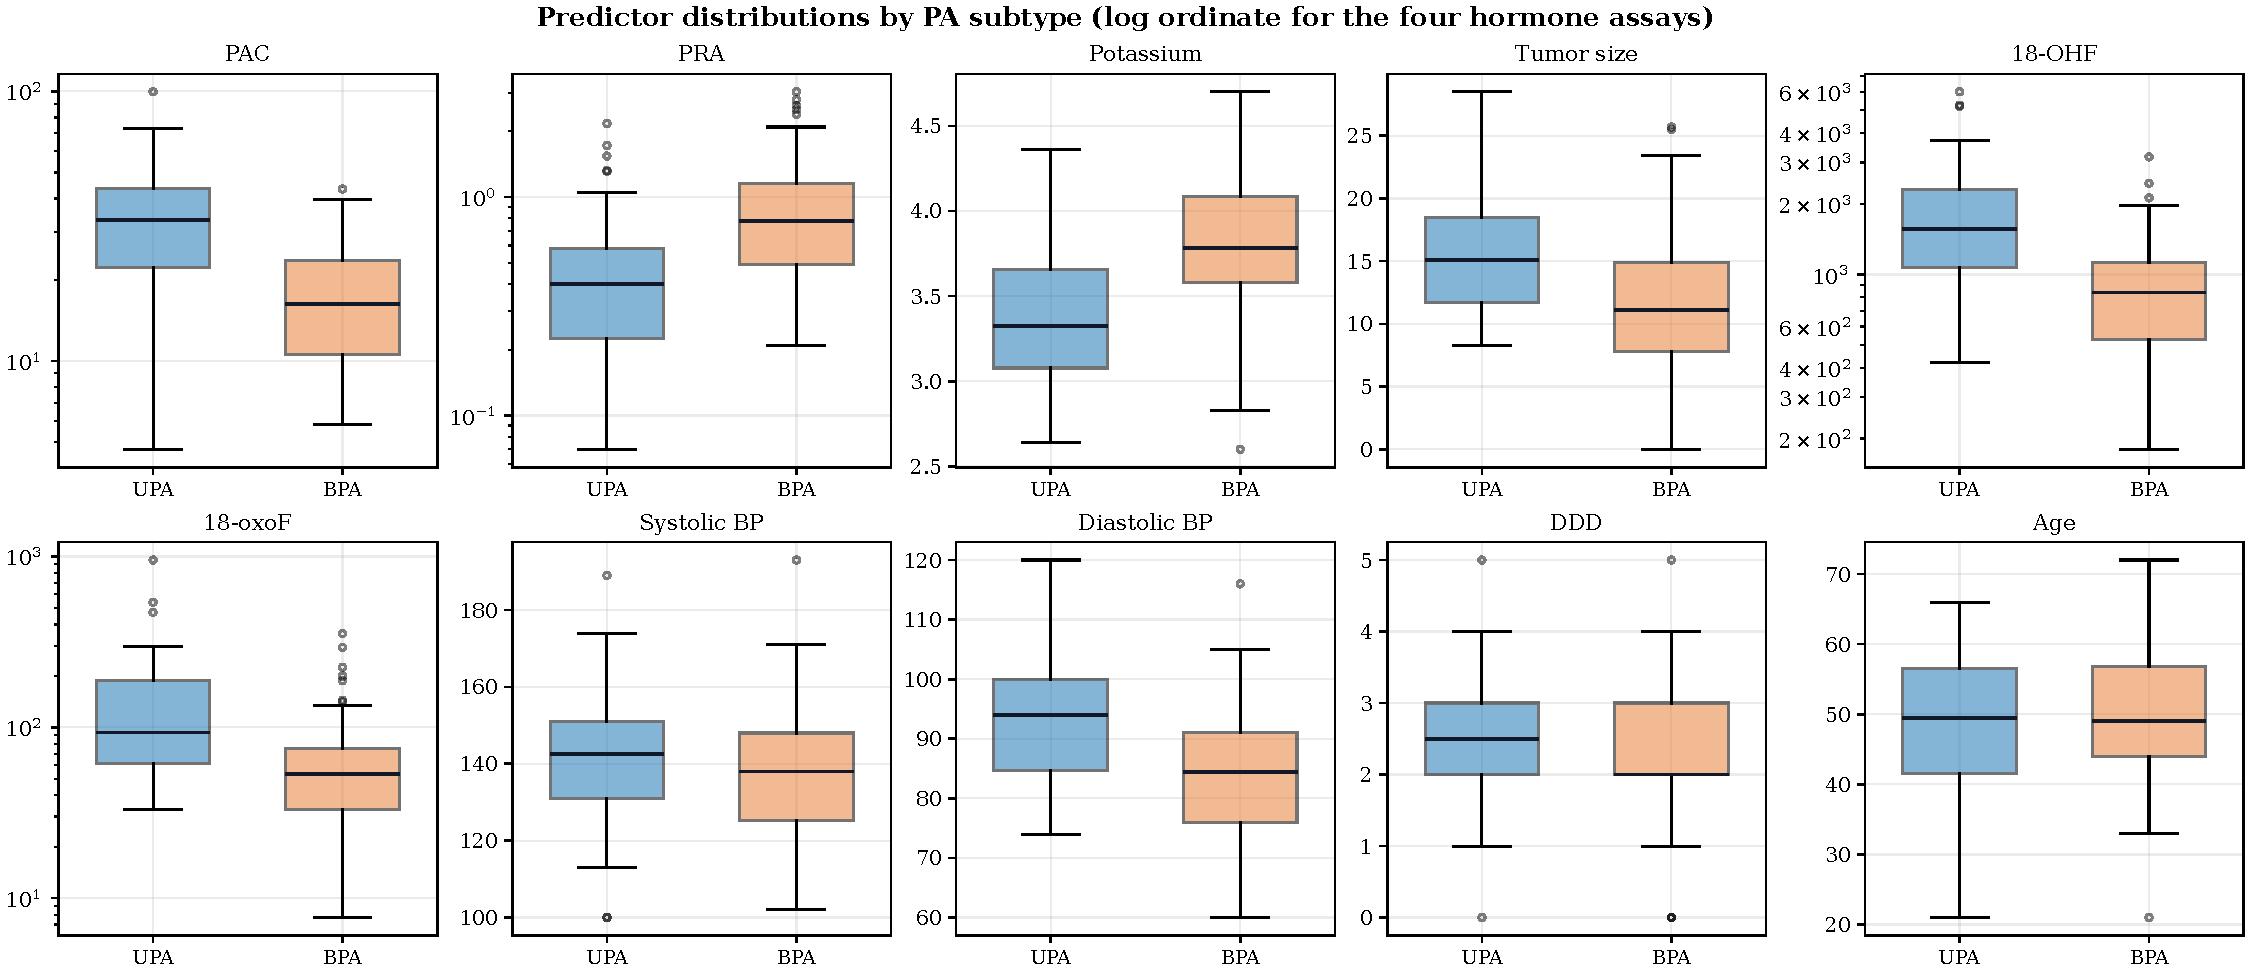
\includegraphics[width=\textwidth]{output/figures/feature_distributions.pdf}
    \caption{Distribution of each predictor by PA subtype. Boxes span the
    interquartile range with the median marked; whiskers extend to
    $1.5\times$IQR and points beyond are drawn individually. The four log transform features (PAC, PRA, 18-OHF, and 18-oxoF) use a logarithmic ordinate to make their right-skewed distributions
    legible. Every panel shows overlapping subtype distributions, which is why
    no single feature (and, as Section~\ref{sec:hard-margin} shows, no
    linear combination of all ten) can separate the classes perfectly.}
    \label{fig:feature-distributions}
\end{figure}

\section{Hard-Margin SVM: Primal, Dual, and Existence}
\label{sec:hard-margin}

\subsection{Primal Optimization Problem}

The linear decision score is $s_i=w^\top x_i+b$, where $w\in\mathbb{R}^p$ is the normal vector of the separating hyperplane and $b\in\mathbb{R}$ is the intercept. The hard-margin primal SVM is the convex quadratic program \cite{cortes1995,lec-statlearn,lec-convex}
\begin{equation}
\begin{aligned}
\min_{w,b}\quad & \phi(w,b)=\frac{1}{2}\lVert w\rVert_2^2\\
\text{subject to}\quad & t_i(w^\top x_i+b)\geq 1,
    \qquad i=1,\ldots,m.
\end{aligned}
\end{equation}
The constraints require every training observation to be correctly classified with functional margin at least one. Minimizing $\lVert w\rVert_2^2/2$ maximizes the geometric margin $2/\lVert w\rVert_2$ between the two supporting hyperplanes \cite{lec-statlearn}.

In a hard-margin SVM there is no per-observation loss term to differentiate. Margin violations are forbidden by constraints rather than assigned a finite loss. Consequently, the quantity differentiated below is the \emph{primal objective}, together with the affine constraint functions.

\subsection{First and Second Derivatives}

Define the augmented parameter vector, quadratic matrix, and signed augmented feature vector as
\begin{equation}
    \theta=\begin{bmatrix}w\\b\end{bmatrix},\qquad
    Q=\begin{bmatrix}I_p&0\\0&0\end{bmatrix},\qquad
    u_i=t_i\begin{bmatrix}x_i\\1\end{bmatrix}.
\end{equation}
The objective and constraints can then be written as
\begin{equation}
    \phi(\theta)=\frac{1}{2}\theta^\top Q\theta,
    \qquad
    g_i(\theta)=1-u_i^\top\theta\leq0.
\end{equation}
The first derivative of the objective is
\begin{equation}
    \nabla\phi(\theta)=Q\theta
    =\begin{bmatrix}w\\0\end{bmatrix},
\end{equation}
and its second derivative is the constant Hessian
\begin{equation}
    \nabla^2\phi(\theta)=Q
    =\begin{bmatrix}I_p&0\\0&0\end{bmatrix}.
\end{equation}
For each margin constraint,
\begin{equation}
    \nabla g_i(\theta)=-u_i
    =-t_i\begin{bmatrix}x_i\\1\end{bmatrix},
    \qquad
    \nabla^2 g_i(\theta)=0.
\end{equation}
Because $Q\succeq0$ and every $g_i$ is affine, the primal problem is convex \cite{lec-convex}. The objective is strictly convex in $w$ but not in the complete vector $(w,b)$ because the intercept is unpenalized. Thus the optimal $w$ is unique whenever a solution exists, whereas the intercept need not be unique. There is also no hinge boundary or nondifferentiable point in this constrained primal formulation.

Section~\ref{sec:worked-excel} evaluates $u_i^\top\theta$ row by row in a ten-observation spreadsheet illustration.

\subsection{Lagrangian and KKT Conditions}

The derivatives of the primal objective describe only how
$\lVert w\rVert_2^2/2$ changes; they do not by themselves enforce the margin
constraints. Indeed, setting the objective gradient to zero would give
$w=0$, which is generally infeasible. The Lagrangian is therefore introduced
as an auxiliary function, not as a replacement for the primal objective, to
combine the objective with the constraints and express constrained
optimality through the KKT conditions.

Introduce one multiplier $\alpha_i\geq0$ for each inequality constraint. The Lagrangian is
\begin{equation}
    \mathcal{L}(w,b,\alpha)
    =\frac{1}{2}\lVert w\rVert_2^2
    +\sum_{i=1}^{m}\alpha_i\left[1-t_i(w^\top x_i+b)\right].
\end{equation}
Its first derivatives with respect to the primal variables are
\begin{equation}
    \nabla_w\mathcal{L}
    =w-\sum_{i=1}^{m}\alpha_i t_i x_i,
    \qquad
    \frac{\partial\mathcal{L}}{\partial b}
    =-\sum_{i=1}^{m}\alpha_i t_i.
\end{equation}
At a stationary point these derivatives vanish, giving
$w=\sum_i\alpha_i t_i x_i$ and $\sum_i\alpha_i t_i=0$. Thus the separating
direction is determined by the training observations whose constraints are
active and whose multipliers are positive, rather than by the unconstrained
minimum $w=0$.

For fixed $\alpha$, the Hessian with respect to $(w,b)$ is again
\begin{equation}
    \nabla^2_{(w,b)}\mathcal{L}
    =\begin{bmatrix}I_p&0\\0&0\end{bmatrix}.
\end{equation}
When the primal is feasible, its Karush--Kuhn--Tucker (KKT) conditions are necessary and sufficient for global optimality \cite{boyd2004,lec-firstorder}:
\begin{equation}
\begin{aligned}
    w-\sum_{i=1}^{m}\alpha_i t_i x_i &=0,
    &\sum_{i=1}^{m}\alpha_i t_i &=0,\\
    t_i(w^\top x_i+b)-1 &\geq0,
    &\alpha_i &\geq0,\\
    \alpha_i\left[t_i(w^\top x_i+b)-1\right]&=0,
    & i&=1,\ldots,m.
\end{aligned}
\end{equation}
The final equality is complementary slackness. Read in both directions it states that an inactive constraint forces a zero multiplier ($t_i(w^\top x_i+b)-1>0\Rightarrow\alpha_i=0$), while a positive multiplier forces an active constraint ($\alpha_i>0\Rightarrow t_i(w^\top x_i+b)=1$); observations with $\alpha_i>0$ therefore lie on a supporting margin and are the support vectors. Complementary slackness is also exactly the term that makes $\sum_i\alpha_i[t_i(w^\top x_i+b)-1]$ vanish in the Lagrangian at optimality, which is what collapses the duality gap to $p^\star=d^\star$ \cite{lec-duality}. Stationarity alone is not sufficient: primal feasibility, dual feasibility, and complementary slackness must also hold.

The KKT conditions are sufficient here because the objective is convex and
the margin constraints are affine. They are also necessary whenever the
hard-margin problem is feasible, for the reason established in
Section~\ref{sec:slater}. Conversely, if the data are not linearly separable,
primal feasibility fails and no triplet $(w,b,\alpha)$ can satisfy the
complete KKT system.

\subsection{Dual Problem and the Meaning of the Dual Bound}

The primal and dual optimize different variables and therefore point in
opposite directions. The primal minimizes over the classifier parameters
$(w,b)$. For any fixed multiplier vector $\alpha\geq0$, define the dual
function as the smallest Lagrangian value attainable by the primal variables,
\begin{equation}
    q(\alpha)=\inf_{w,b}\mathcal{L}(w,b,\alpha).
\end{equation}
For every primal-feasible $(w,b)$, the constraint terms
$1-t_i(w^\top x_i+b)$ are nonpositive. Hence
\begin{equation}
    q(\alpha)\leq \mathcal{L}(w,b,\alpha)
    \leq \frac12\lVert w\rVert_2^2.
\end{equation}
Thus each dual-feasible $\alpha$ supplies a \emph{lower bound} on every
feasible primal objective value. This is the dual bound, the weak-duality
inequality of \cite{lec-duality}. The dual maximizes
$q(\alpha)$ because it seeks the largest, and therefore tightest, lower bound;
this explains why the primal is a minimization problem while the dual is a
maximization problem.

Using stationarity,
$w=\sum_i\alpha_i t_i x_i$ and $\sum_i\alpha_i t_i=0$, eliminates $w$ and
$b$ from the Lagrangian and gives
\begin{equation}
\begin{aligned}
\max_{\alpha}\quad
&q(\alpha)=\sum_{i=1}^{m}\alpha_i
-\frac12\sum_{i=1}^{m}\sum_{j=1}^{m}
  \alpha_i\alpha_j t_i t_j x_i^\top x_j\\
\text{subject to}\quad
&\alpha_i\geq0,\qquad
\sum_{i=1}^{m}\alpha_i t_i=0.
\end{aligned}
\end{equation}
Weak duality always gives $d^*\leq p^*$. Whether that inequality tightens to
an equality is a separate question, settled by the constraint qualification of
the next subsection.

\subsection{Slater's Condition and Strong Duality}
\label{sec:slater}

Weak duality is automatic, but the dual is a faithful stand-in for the primal
only when the gap closes \cite{lec-duality}. For a convex program
\begin{equation}
\begin{aligned}
\min_{x}\quad & f(x)\\
\text{subject to}\quad & f_i(x)\leq0,\qquad i=1,\ldots,m,\\
& Ax=b,
\end{aligned}
\end{equation}
\emph{Slater's constraint qualification} asks for a strictly feasible point:
some $\tilde{x}\in\operatorname{int}\mathcal{D}$ with
\begin{equation}
    f_i(\tilde{x})<0 \quad\text{for all } i=1,\ldots,m,
    \qquad A\tilde{x}=b,
\end{equation}
where $A$ has full row rank. When it holds, $p^*=d^*$; and if $d^*>-\infty$,
the dual optimum is attained \cite{boyd2004}.

Two refinements decide the matter here. The strict inequality is needed only
for the \emph{non-affine} inequality constraints, so for a convex program
whose inequality constraints are all affine, Slater's condition collapses to
ordinary feasibility.

That is precisely the present case. The objective
$\frac12\lVert w\rVert_2^2$ is convex and every margin constraint
$1-t_i(w^\top x_i+b)\leq0$ is affine in $(w,b)$, so strong duality holds for
the hard-margin SVM as soon as one separating hyperplane exists. Feasibility is therefore the single hinge of the entire hard-margin
analysis. The certificate of Section~\ref{sec:full-certificate} shows the
constraints are infeasible on this dataset, so $p^*=+\infty$ and there is no
finite primal value for the dual to certify, which is why a dual solution
must never be read as a trained classifier before feasibility is checked.

The soft-margin program of Section~\ref{sec:soft-margin} differs in exactly
the way that matters. Its constraints
$1-\xi_i-t_i(w^\top x_i+b)\leq0$ and $-\xi_i\leq0$ are again affine, and the
point $(w,b,\xi)=(0,0,\mathbf{1})$ is feasible for \emph{any} dataset.
Slater's condition therefore holds unconditionally, strong duality is
guaranteed in advance, and the vanishing primal--dual gaps reported later
($4.9\times10^{-10}$ for the linear model, $2.2\times10^{-11}$ for the RBF
model) are genuine checks on solver accuracy rather than assumptions being
taken on trust.

\subsection{Linear Separability and Existence of a Hard-Margin Solution}

Let $U\in\mathbb{R}^{m\times(p+1)}$ have rows
$u_i^\top=t_i[x_i^\top,1]$ and let
$\theta=[w^\top,b]^\top$. A hard-margin solution exists if and only if the
linear system
\begin{equation}
    U\theta\geq\mathbf{1}
\end{equation}
is feasible. This condition is also equivalent to strict linear separability:
if some hyperplane correctly separates all observations with strictly positive
signed scores, rescaling $(w,b)$ makes the smallest signed score equal to one;
conversely, any point satisfying the unit-margin inequalities is a strict
separator.

The existence question is checked by the zero-objective linear program
\begin{equation}
    \min_{\theta}\;0
    \qquad\text{subject to}\qquad
    -U\theta\leq-\mathbf{1}.
\end{equation}
If it is feasible, its output supplies a valid starting point for minimizing
the quadratic primal objective. If it is infeasible, changing the objective
from zero to $\lVert w\rVert_2^2/2$ cannot make the empty feasible set nonempty:
the hard-margin primal has no solution. This logical order separates two
questions that are often confused: feasibility asks whether any separating
hyperplane exists, whereas optimization selects the maximum-margin hyperplane
only after existence has been established.

Two worked numerical examples are provided in Appendix~\ref{app:worked-examples}. They illustrate feasible hard-margin primal--dual calculations without interrupting the full-cohort feasibility argument.

\section{Hard-Margin Feasibility Audit and Certificate}

\subsection{Full-Data Infeasibility Certificate}
\label{sec:full-certificate}

Three mutually reinforcing checks are used on the complete processed dataset,
in the order direct solver status, algebraic Farkas certificate, and geometric
convex-hull interpretation. Here
$U\in\mathbb{R}^{114\times11}$ contains the ten standardized features and the
intercept column.

\paragraph{Direct full-data feasibility check.}
The primal model supplied to a constrained solver is
\begin{equation}
\begin{aligned}
\min_{w,b}\quad &\frac12\lVert w\rVert_2^2\\
\text{subject to}\quad &U\theta\geq\mathbf{1}.
\end{aligned}
\end{equation}
Before an objective can be minimized, the solver must find a point satisfying
all 114 constraints. The implementation therefore first solves the equivalent
feasibility model $\min_\theta 0$ subject to $-U\theta\leq-\mathbf{1}$; changing
the objective cannot make an empty feasible set nonempty. The direct solver
audit returned the result in Table~\ref{tab:direct-solver}.

\begin{table}[htbp]
\centering
\caption{Direct full-data primal feasibility check.}
\label{tab:direct-solver}
\begin{tabular}{ll}
\toprule
Item & Solver result \\
\midrule
Decision variables $(w_1,\ldots,w_{10},b)$ & 11 \\
Hard-margin constraints & 114 \\
Solver & SciPy HiGHS \\
HiGHS model status & Status 8: Infeasible \\
Primal parameters $(w,b)$ returned & None \\
Primal objective $\frac12\lVert w\rVert_2^2$ & Not defined \\
\bottomrule
\end{tabular}

\end{table}

Thus the correct statement is that the solver returns an \emph{infeasible
status}; it does not return an ``infeasible solution.'' No primal solution
exists for the solver to report. This is the direct computational verification
used in the direct verification workflow. In the corresponding hard-margin
dual, primal infeasibility means that no finite primal optimum exists to be
matched by a valid classifier. Indeed, scaling the Farkas vector below gives a
dual-feasible ray with zero quadratic term and an arbitrarily large linear
term, so the hard-margin dual is unbounded above; it cannot rescue the empty
primal feasible set.

\paragraph{Independent certificate.}
The solver status is then strengthened by a direct, independently checkable
proof. Farkas' lemma states that the system
$U\theta\geq\mathbf{1}$ is infeasible if and only if there is a vector
$\lambda\in\mathbb{R}^{114}$ satisfying
\begin{equation}
    \lambda\geq0,\qquad
    U^\top\lambda=0,\qquad
    \mathbf{1}^\top\lambda=1.
\end{equation}
The auxiliary linear program for this certificate returned twelve nonzero
weights, shown in Table~\ref{tab:farkas-certificate}; the other 102 weights
are zero. The displayed values alone should not be used to recompute the
certificate; every check uses the unrounded values in the companion CSV file.

\begin{table}[htbp]
\centering
\caption{Nonzero weights in the full-data Farkas infeasibility certificate.}
\label{tab:farkas-certificate}
\scriptsize
\begin{tabular}{llr@{\qquad}llr}
\toprule
Patient & Class & $\lambda_i$ & Patient & Class & $\lambda_i$ \\
\midrule
CGH-021 & UPA & 0.21 & CGH-072 & BPA & 0.04 \\
CGH-024 & BPA & 0.05 & CGH-081 & UPA & 0.01 \\
CGH-026 & BPA & 0.16 & CGH-092 & BPA & 0.01 \\
CGH-053 & UPA & 0.04 & CGH-105 & UPA & 0.01 \\
CGH-058 & UPA & 0.17 & CGH-108 & BPA & 0.05 \\
CGH-060 & BPA & 0.18 & CGH-111 & UPA & 0.07 \\
\bottomrule
\end{tabular}

\end{table}

The full-precision numerical audit gives
\begin{equation}
\begin{aligned}
\mathbf{1}^\top\lambda&=1.00,\\
\sum_{i:t_i=+1}\lambda_i&=0.50,\\
\sum_{i:t_i=-1}\lambda_i&=0.50,\\
\lVert U^\top\lambda\rVert_\infty&<10^{-15}.
\end{aligned}
\end{equation}
The final residual is reported
as a tolerance statement because its exact machine-zero mantissa can change
with the numerical backend. Now suppose, for
contradiction, that a hard-margin parameter $\theta$ satisfied
$U\theta\geq\mathbf{1}$. Nonnegativity of $\lambda$ would imply
\begin{equation}
\underbrace{(U^\top\lambda)^\top\theta}_{0}
=\lambda^\top U\theta
\geq\lambda^\top\mathbf{1}
=1,
\end{equation}
which is the contradiction $0\geq1$. Therefore the complete hard-margin
constraint system has no feasible solution. In fact, the twelve observations
in Table~\ref{tab:farkas-certificate} already provide a sufficient
infeasible subsystem.

The same certificate has a geometric interpretation. Because the intercept
component of $U^\top\lambda=0$ gives equal class masses of $0.5$, define
$\beta_i^+=2\lambda_i$ for UPA and $\beta_i^-=2\lambda_i$ for BPA. Each set of
coefficients is nonnegative and sums to one, while the feature components of
$U^\top\lambda=0$ give
\begin{equation}
    \sum_{i:t_i=+1}\beta_i^+x_i
    =\sum_{i:t_i=-1}\beta_i^-x_i.
\end{equation}
Thus the standardized UPA and BPA convex hulls contain the same point. Their
largest coordinate difference is below $10^{-15}$ (machine precision), as illustrated
in Figure~\ref{fig:full-certificate}. Intersecting convex hulls cannot be
strictly separated by a hyperplane.

\begin{figure}[htbp]
    \centering
    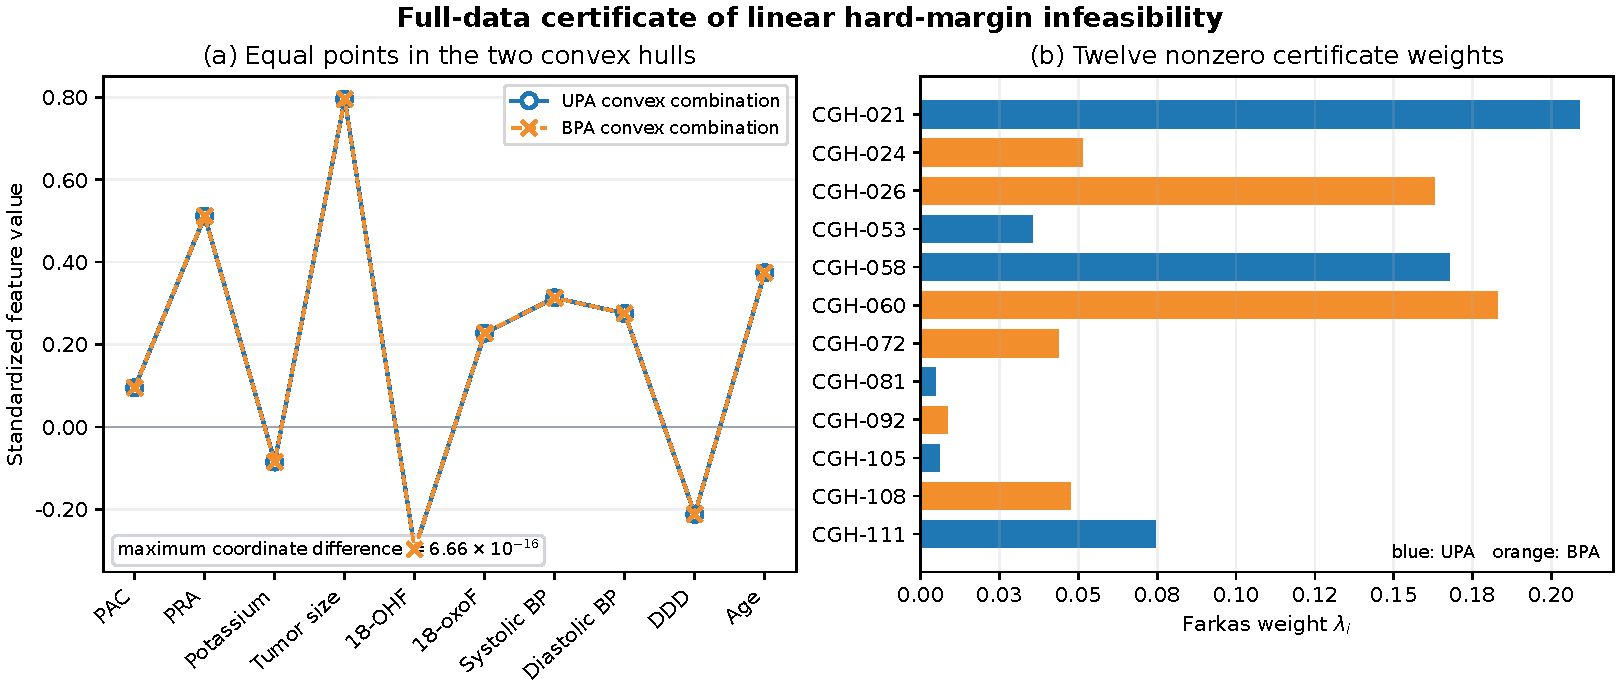
\includegraphics[width=0.98\textwidth]{output/figures/full_data_infeasibility_certificate.pdf}
    \caption{Full-data infeasibility certificate. Panel (a) shows the identical ten-dimensional point obtained as a convex combination of UPA observations and as a convex combination of BPA observations; the plot compares coordinates directly and is not a two-dimensional projection. Panel (b) shows the twelve nonzero Farkas weights.}
    \label{fig:full-certificate}
\end{figure}

Two complementary illustrations make the certificate intuitive.
Figure~\ref{fig:farkas-schematic} contrasts the two systems of Farkas' lemma:
either a separating hyperplane exists (System~A), or a nonnegative combination
of the constraints proves a contradiction $0\ge1$ (System~B), never both.
Figure~\ref{fig:hull-overlap} provides a two-dimensional visual intuition by
projecting the project data onto its first two principal components. The
projected convex hulls overlap, which is consistent with---but does not by
itself prove---nonseparability in the original ten-dimensional space. The
proof is the full-dimensional Farkas certificate above. The
theory-of-the-alternative structure behind this argument
follows the treatment of duality and first-order optimality in the course
lectures \cite{lec-duality,lec-firstorder}.

\begin{figure}[htbp]
    \centering
    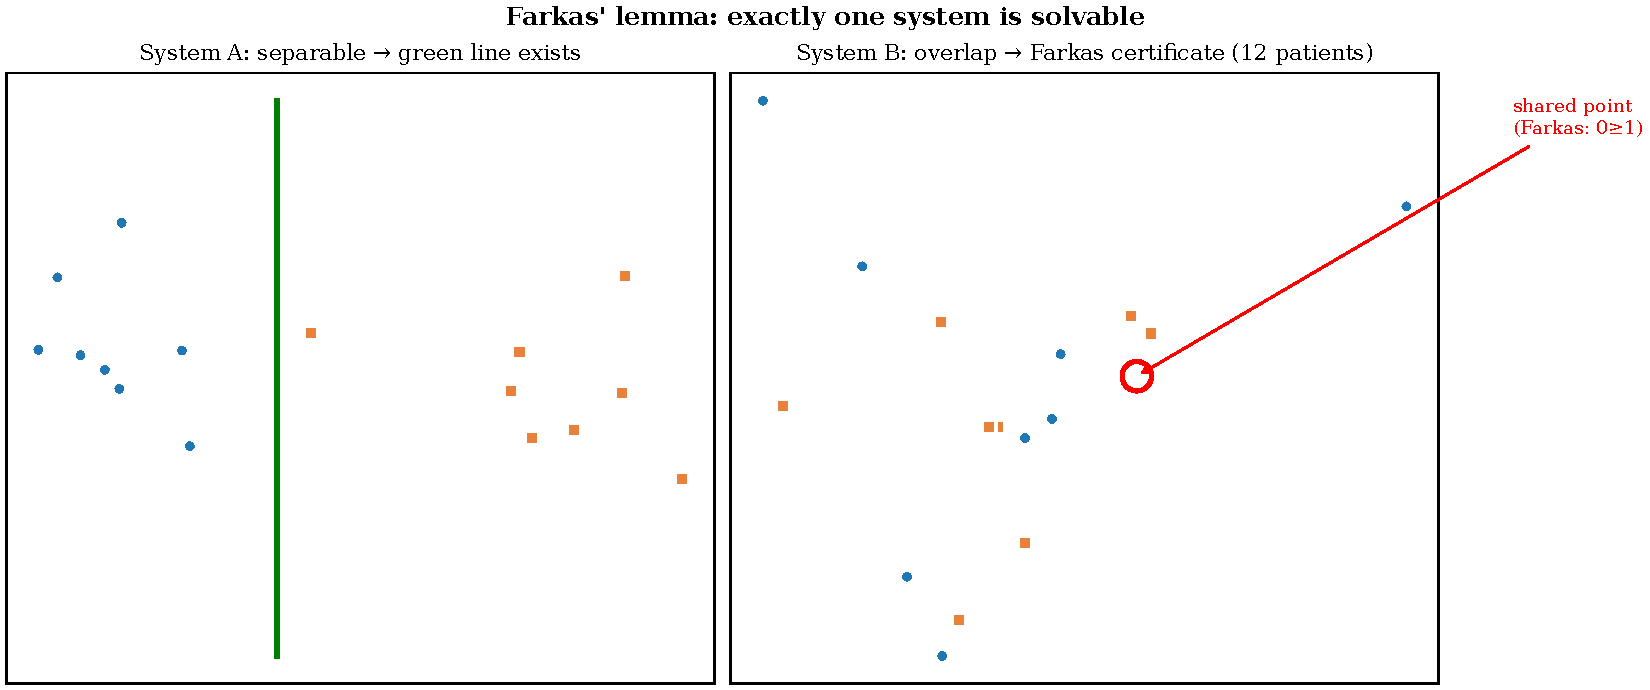
\includegraphics[width=0.95\textwidth]{output/figures/farkas_lemma_schematic.pdf}
    \caption{Farkas' lemma as a theorem of the alternative. System~A (left): the
    classes are separable, so a hyperplane exists. System~B (right): the classes
    overlap, so a nonnegative weighting of the points certifies infeasibility
    ($0\ge1$). Exactly one system is solvable; for the project data it is
    System~B.}
    \label{fig:farkas-schematic}
\end{figure}

\begin{figure}[htbp]
    \centering
    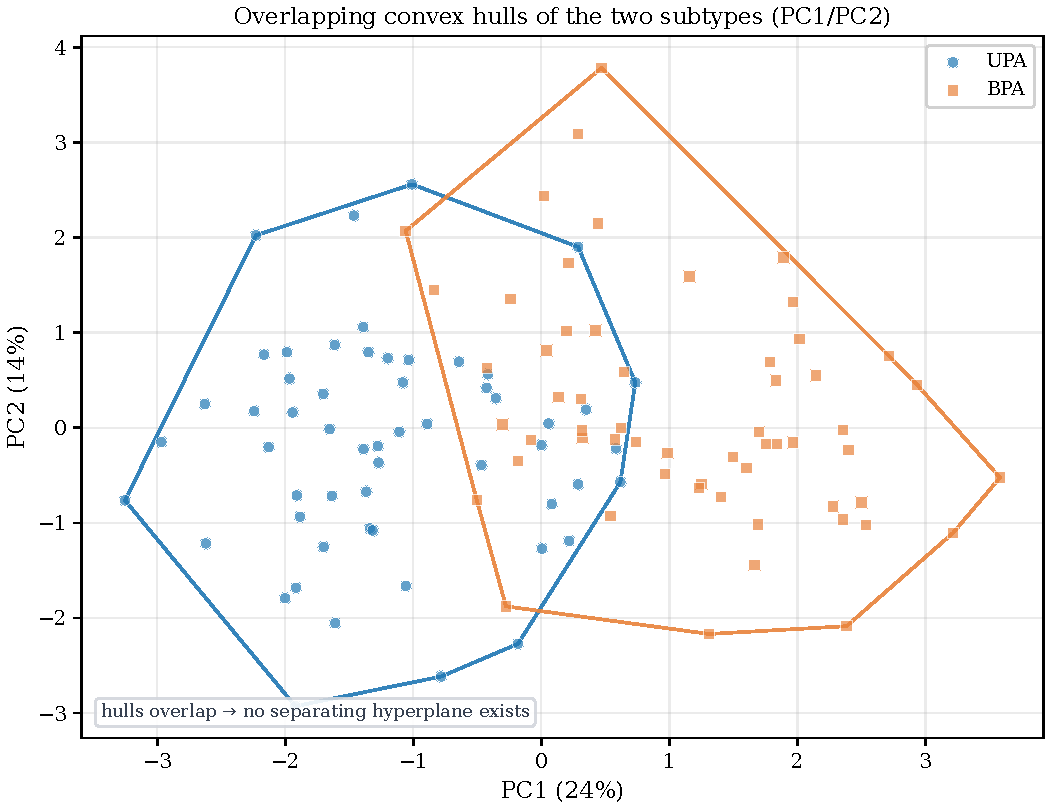
\includegraphics[width=0.72\textwidth]{output/figures/convex_hull_overlap_2d.pdf}
    \caption{Convex hulls of the UPA and BPA subtypes in the first two principal
    components of the standardized data. Their overlap illustrates the class
    mixing visible in this projection but does not establish nonseparability in
    ten dimensions. The full-dimensional certificate in
    Figure~\ref{fig:full-certificate} provides that proof.}
    \label{fig:hull-overlap}
\end{figure}

Consequently, for the current preprocessed project data,
\begin{equation}
\boxed{\text{the UPA and BPA classes are not linearly separable in this processed representation}.}
\end{equation}
The qualification matters: the log transform is nonlinear, so this certificate
does not make a claim about every alternative representation of the raw data.
Nor does linear nonseparability preclude separation after a nonlinear kernel
map; it establishes only that the stated linear hard-margin problem is empty.
The certificate, CSV output, numerical checks, and figure are reproduced by
\path{scripts/build_full_data_infeasibility_certificate.py}. The script writes
four machine-readable audit files under \path{output/csv/}: the direct solver
status, sparse Farkas vector, two convex-hull representations, and numerical
residual checks. The two tables above are generated from the same Python
results and then included in this PDF.

\subsection{Cross-Validation Feasibility Results and ROC Rule}

The feasibility audit uses stratified five-fold cross-validation with shuffling and random seed zero. All preprocessing operations are fitted inside the training fold. In each fold, the hard-margin classifier is fitted only if the training constraints are feasible. Held-out decision scores would then be pooled to construct the ROC curve, and AUROC would summarize discrimination across score thresholds.

\begin{table}[htbp]
\centering
\caption{Hard-margin feasibility results for the full synthetic cohort and
the five cross-validation training folds. ``No'' means that no parameter pair
$(w,b)$ satisfies every unit-margin constraint in that row's training set.}
\label{tab:feasibility}
\begin{tabular}{lrrc}
\toprule
Data split & Training observations & Held-out observations & Feasible \\
\midrule
Full dataset & 114 & -- & No \\
Fold 1 & 91 & 23 & No \\
Fold 2 & 91 & 23 & No \\
Fold 3 & 91 & 23 & No \\
Fold 4 & 91 & 23 & No \\
Fold 5 & 92 & 22 & No \\
\bottomrule
\end{tabular}

\end{table}

The result is unambiguous: the full-data problem is infeasible, and all five
training-fold problems are also infeasible. Thus linear separation is not
available in any evaluated hard-margin fit; there are no valid hard-margin
parameters with which to score the corresponding held-out observations.

This ordering is important. ROC analysis requires a fitted scoring function for every held-out observation. If a training fold is infeasible, there are no valid hard-margin parameters for that fold and therefore no legitimate out-of-fold scores. Reporting an ROC curve in that situation would require silently changing either the model or the data.

The worked subsystem in Section~\ref{sec:worked-excel} is not a cross-validation split and is not used to generate ROC results.

The hard-margin question is therefore closed: the complete cohort and every
training fold are infeasible, so the model cannot be fitted or evaluated by
ROC analysis. Section~\ref{sec:soft-margin} now relaxes the unit-margin
constraints explicitly by introducing penalized slack variables.

\section{Linear Soft-Margin SVM}
\label{sec:soft-margin}

\subsection{Why Slack Variables Are Needed}

The preceding hard-margin audit, including the certificate in
Section~\ref{sec:full-certificate}, establishes that no $(w,b)$ can satisfy
all 114 unit-margin inequalities simultaneously. The soft-margin model changes the
assumption rather than attempting to optimize over an empty set. For each
observation it introduces a slack variable $\xi_i\geq0$ that measures the
shortfall from the desired signed functional margin of one:
\begin{equation}
    \xi_i=\max\{0,1-t_i(w^\top x_i+b)\}.
\end{equation}
When $\xi_i=0$, the observation lies on or outside its supporting margin. If
$0<\xi_i\leq1$, it lies inside the margin but remains on the correct side of
the decision boundary. If $\xi_i>1$, its signed score is negative and it is
misclassified. This interpretation directly connects the optimization
variables to the geometry of overlapping UPA and BPA observations.

\subsection{Soft-Margin Primal Problem}

The linear soft-margin primal problem is \cite{cortes1995,lec-statlearn}
\begin{equation}
\begin{aligned}
\min_{w,b,\xi}\quad
&p(w,b,\xi)=\frac12\lVert w\rVert_2^2+C\sum_{i=1}^{m}\xi_i\\
\text{subject to}\quad
&t_i(w^\top x_i+b)\geq1-\xi_i,\qquad i=1,\ldots,m,\\
&\xi_i\geq0,\qquad i=1,\ldots,m.
\end{aligned}
\end{equation}
The first term favors a wide margin, while the second penalizes total margin
violation. The constant $C>0$ controls their trade-off. Unlike the hard-margin
problem, this primal is always feasible: $w=0$, $b=0$, and $\xi_i=1$ satisfy
every constraint. Eliminating the slack variables gives the equivalent
unconstrained hinge-loss form
\begin{equation}
    \min_{w,b}\quad
    \frac12\lVert w\rVert_2^2
    +C\sum_{i=1}^{m}\max\{0,1-t_i(w^\top x_i+b)\}.
\end{equation}
The constrained form is retained below because it makes the primal--dual
relationship and the role of $C$ explicit.

\subsection{Lagrangian and KKT Conditions}

Introduce $\alpha_i\geq0$ for
$1-\xi_i-t_i(w^\top x_i+b)\leq0$ and $\mu_i\geq0$ for
$-\xi_i\leq0$. The Lagrangian is
\begin{equation}
\begin{aligned}
\mathcal{L}(w,b,\xi,\alpha,\mu)
={}&\frac12\lVert w\rVert_2^2+C\sum_i\xi_i\\
&+\sum_i\alpha_i[1-\xi_i-t_i(w^\top x_i+b)]
-\sum_i\mu_i\xi_i.
\end{aligned}
\end{equation}
Stationarity with respect to the primal variables gives
\begin{equation}
    w=\sum_i\alpha_i t_i x_i,\qquad
    \sum_i\alpha_i t_i=0,\qquad
    C-\alpha_i-\mu_i=0.
\end{equation}
Because $\mu_i\geq0$, the final equality produces the upper bound
$0\leq\alpha_i\leq C$. The complete KKT system additionally requires primal
feasibility, dual feasibility, and complementary slackness:
\begin{equation}
\begin{aligned}
&t_i(w^\top x_i+b)-1+\xi_i\geq0,\qquad \xi_i\geq0,\\
&0\leq\alpha_i\leq C,\\
&\alpha_i[1-\xi_i-t_i(w^\top x_i+b)]=0,\\
&(C-\alpha_i)\xi_i=0.
\end{aligned}
\end{equation}
These conditions are necessary and sufficient because the primal objective is
convex, its constraints are affine, and strict feasibility is obtained by
choosing sufficiently large positive slacks. They also explain the support
vectors. An observation with $\alpha_i=0$ does not determine $w$ and lies
outside the margin. A point with $0<\alpha_i<C$ lies exactly on a supporting
margin. A point with $\alpha_i=C$ may lie inside the margin or be
misclassified, so it receives the largest multiplier permitted by the chosen
penalty.

\subsection{Soft-Margin Dual Problem}

Minimizing the Lagrangian over $w$, $b$, and $\xi$ using the stationarity
conditions yields
\begin{equation}
\begin{aligned}
\max_{\alpha}\quad
&d(\alpha)=\sum_{i=1}^{m}\alpha_i
-\frac12\sum_{i=1}^{m}\sum_{j=1}^{m}
\alpha_i\alpha_jt_it_jx_i^\top x_j\\
\text{subject to}\quad
&0\leq\alpha_i\leq C,\qquad
\sum_{i=1}^{m}\alpha_it_i=0.
\end{aligned}
\end{equation}
The objective has the same form as the hard-margin dual, but the new box
constraint $\alpha_i\leq C$ is essential. It prevents any single observation
from exerting unlimited pressure on the separating hyperplane. Since the
soft-margin primal is strictly feasible, strong duality holds and the optimal
primal and dual values are equal up to numerical solver tolerance.

\subsection{Selecting the Penalty Parameter by Grid Search}

A small $C$ places greater emphasis on a wide, strongly regularized margin and
accepts more slack. A large $C$ penalizes violations more severely and moves
toward hard-margin behavior, which can increase sensitivity to overlapping
observations. Because neither extreme is known in advance, $C$ is selected
from the half-logarithmic grid
\begin{equation}
\mathcal{C}=\{10^{k/2}:k=-4,-3,\ldots,4\}.
\end{equation}
Displayed to two decimal places, these values are
\begin{equation}
0.01,\ 0.03,\ 0.10,\ 0.32,\ 1.00,\ 3.16,\ 10.00,\ 31.62,\ 100.00.
\end{equation}
Each candidate is evaluated by mean five-fold stratified validation AUROC.
The log transformation, median imputation, standardization, and linear SVM
are placed in one pipeline, so every preprocessing parameter is estimated
from the corresponding training fold only.

There are therefore two distinct optimization levels. For a fixed candidate
$C$ and training fold $r$, the SMO solver first finds the optimal model for
that value alone:
\begin{equation}
 (w^*_{C,r},b^*_{C,r},\xi^*_{C,r})
 =\arg\min_{w,b,\xi}
 \left\{\frac12\lVert w\rVert^2+C\sum_{i\in\mathcal T_r}\xi_i\right\}
 \quad\text{subject to the fold's soft-margin constraints.}
\end{equation}
That optimized model scores validation fold $\mathcal V_r$. Grid search then
selects the hyperparameter by
\begin{equation}
 \widehat C
 =\arg\max_{C\in\mathcal C}\frac15\sum_{r=1}^{5}
 \operatorname{AUROC}\!\left(\mathcal V_r;w^*_{C,r},b^*_{C,r}\right).
\end{equation}
Thus every candidate $C$ has its own fully optimized coefficients in every
fold; $C$ is compared using held-out AUROC, not by comparing training
objective values across different penalties. After $\widehat C$ is chosen,
the pipeline solves once more at that fixed value using all observations
available to that stage.

Nested cross-validation separates model selection from performance
estimation. In each of five outer folds, an independent five-fold inner grid
search chooses $C$ using only the outer training observations. The selected
model then scores the untouched outer test fold. Table~\ref{tab:soft-nested}
shows that all five inner searches selected $C=0.01$.
Because the same seed-zero outer partition is also used to draw the fixed-$C$
validation curve, and every inner search selected the same $C$, its five test
fold AUROCs numerically coincide with the corresponding fixed-$C$ fold scores.
The nesting remains methodologically valid---each outer test fold is untouched
by selection---but the numerical coincidence is not independent corroborating
evidence.

\begin{table}[htbp]
\centering
\caption{Nested cross-validation for soft-margin penalty selection. AUROC values and $C$ are displayed to two decimal places.}
\label{tab:soft-nested}
\small
\begin{tabular}{rrrrrr}
\toprule
Outer fold & Train & Test & Selected $C$ & Inner AUROC & Outer AUROC \\
\midrule
1 & 91 & 23 & 0.01 & 0.95 & 0.92 \\
2 & 91 & 23 & 0.01 & 0.96 & 0.95 \\
3 & 91 & 23 & 0.01 & 0.94 & 0.98 \\
4 & 91 & 23 & 0.01 & 0.91 & 0.98 \\
5 & 92 & 22 & 0.01 & 0.95 & 0.89 \\
Mean & --- & --- & --- & 0.941 & 0.945 \\
\bottomrule
\end{tabular}

\end{table}

\subsection{Soft-Margin Solution on the Project Dataset}

The final full-data grid search also selected $C=0.01$, with mean five-fold
validation AUROC $0.95$. Figure~\ref{fig:soft-grid-roc} shows both the validation
curve over $C$ and the nested out-of-fold ROC curve. Across the five untouched
outer folds in this illustrative seed-zero partition, mean fold-wise AUROC is
$0.95$; pooling all
out-of-fold scores gives AUROC $0.95$, with accuracy, sensitivity, and
specificity all approximately $0.86$ at decision threshold zero. These
numbers are generated by the explicit linear soft-margin primal--dual model
defined in this section.

The fitted standardized-space coefficients in
Table~\ref{tab:soft-coefficients} give the final linear scoring function.
Their signs describe the direction of the score after the stated preprocessing
but should not be interpreted as causal clinical effects.

\begin{table}[H]
\centering
\caption{Final standardized-space soft-margin coefficients at $C=0.01$.}
\label{tab:soft-coefficients}
\begin{tabular}{lr@{\qquad}lr}
\toprule
Parameter & Estimate & Parameter & Estimate \\
\midrule
PAC & 0.29 & 18-oxoF & 0.22 \\
PRA & -0.18 & Systolic BP & 0.09 \\
Potassium & -0.19 & Diastolic BP & 0.18 \\
Tumor size & 0.15 & DDD & 0.07 \\
18-OHF & 0.23 & Age & -0.08 \\
Intercept & -0.02 & & \\
\bottomrule
\end{tabular}

\end{table}

\begin{figure}[H]
    \centering
    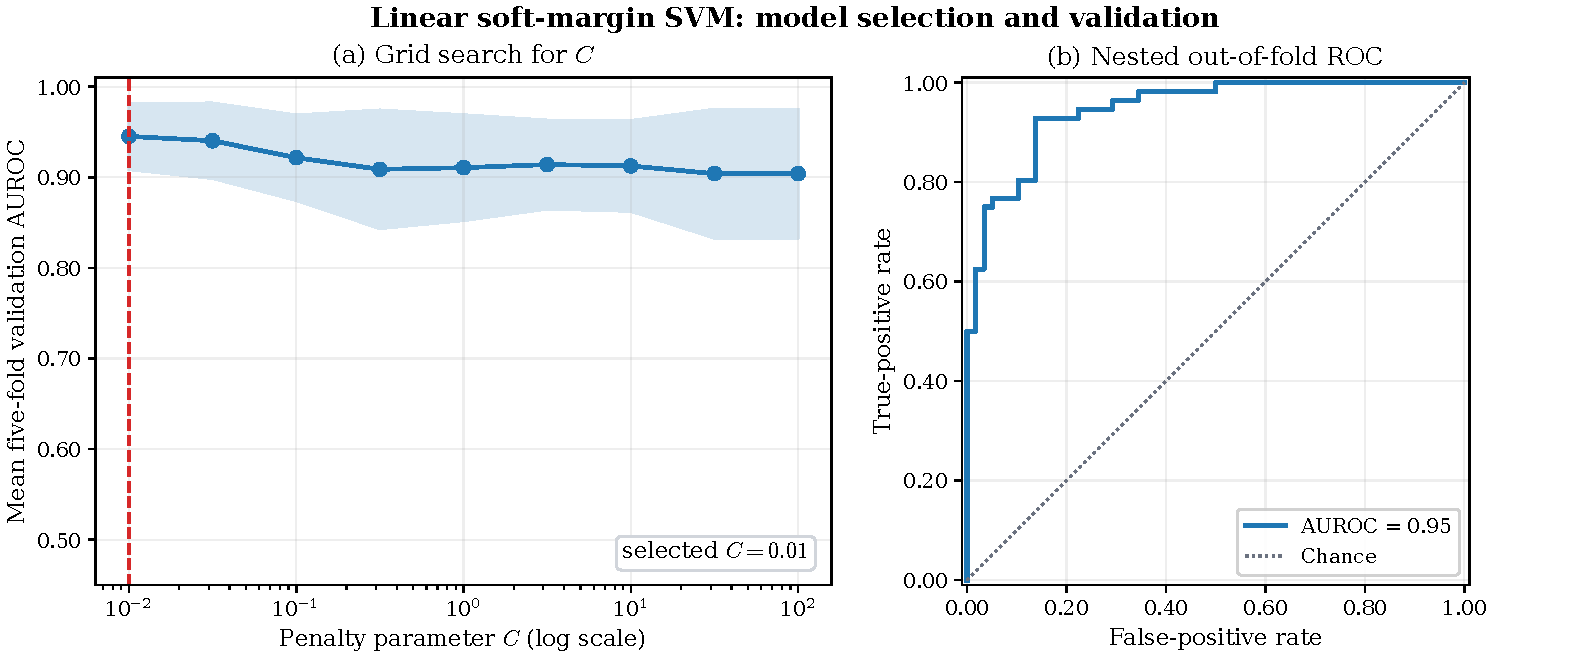
\includegraphics[width=0.98\textwidth]{output/figures/linear_soft_margin_grid_roc.pdf}
    \caption{Soft-margin model selection and validation. Panel (a) reports mean five-fold validation AUROC with one population standard deviation across folds ($\mathrm{ddof}=0$) for every candidate $C$; the dashed line marks the selected value. Panel (b) reports the nested out-of-fold ROC obtained when $C$ is selected inside each outer training fold.}
    \label{fig:soft-grid-roc}
\end{figure}

The full-data solution contains 82 support vectors and 77 observations with
positive slack, with $\sum_i\xi_i=46.89$. Substitution into the primal gives
\begin{equation}
\begin{aligned}
p^*
&=\frac12\lVert w\rVert_2^2+C\sum_i\xi_i\\
&=\frac12(0.33)+(0.01)(46.89)\\
&\approx0.63.
\end{aligned}
\end{equation}
The dual calculation gives $d^*\approx0.63$, and the full-precision
primal--dual gap is $4.85\times10^{-10}$. The weight-reconstruction residual
is zero at stored precision. The dual equality residual is below $10^{-15}$ and
can vary slightly with floating-point summation order. The two maximum
complementary-slackness residuals are $2.35\times10^{-10}$ and
$8.57\times10^{-11}$, confirming the
KKT conditions to solver tolerance. Table~\ref{tab:soft-summary} summarizes
the model-selection and optimization results.

\begin{table}[H]
\centering
\caption{Soft-margin model-selection, validation, and optimization summary
for the prespecified seed-zero split.}
\label{tab:soft-summary}
\begin{tabular}{lr}
\toprule
Quantity & Value \\
\midrule
Selected $C$ from full-data grid search & 0.01 \\
Mean inner-CV AUROC at selected $C$ & 0.95 \\
Nested out-of-fold AUROC & 0.95 \\
Nested out-of-fold accuracy & 0.86 \\
Nested sensitivity & 0.86 \\
Nested specificity & 0.86 \\
Full-data support vectors & 82 \\
Full-data observations with $\xi_i>0$ & 77 \\
Full-data $\sum_i\xi_i$ & 46.89 \\
Full-data primal objective & 0.63 \\
Full-data dual objective & 0.63 \\
\bottomrule
\end{tabular}

\end{table}

All full-precision grid-search results, nested predictions, coefficients,
support-vector multipliers, slacks, and primal--dual checks are written under
\path{output/csv/} by \path{scripts/linear_soft_margin_svm.py}. Tables in this
section and both panels of Figure~\ref{fig:soft-grid-roc} are generated from
those Python outputs.

The penalty $C$ is selected by the grid search of Figure~\ref{fig:c-grid}:
validation AUROC is highest at the strongly regularized end and the
training--validation gap is smallest there, so $C=0.01$ is preferred.
Figure~\ref{fig:soft-pareto} recasts the same grid as a Pareto trade-off
between validation performance and overfitting, on which $C=0.01$ is the single
non-dominated point within the prespecified grid. These AUROC differences are
small relative to the fold-to-fold standard deviations and should not be read
as precise evidence that adjacent settings differ. Figure~\ref{fig:soft-boundary} shows the resulting
soft-margin boundary in the first two principal components: the separating line
passes straight through the region where the two subtypes overlap, accepting
the misclassifications it cannot avoid and charging for them through the slack
variables.

\begin{figure}[htbp]
    \centering
    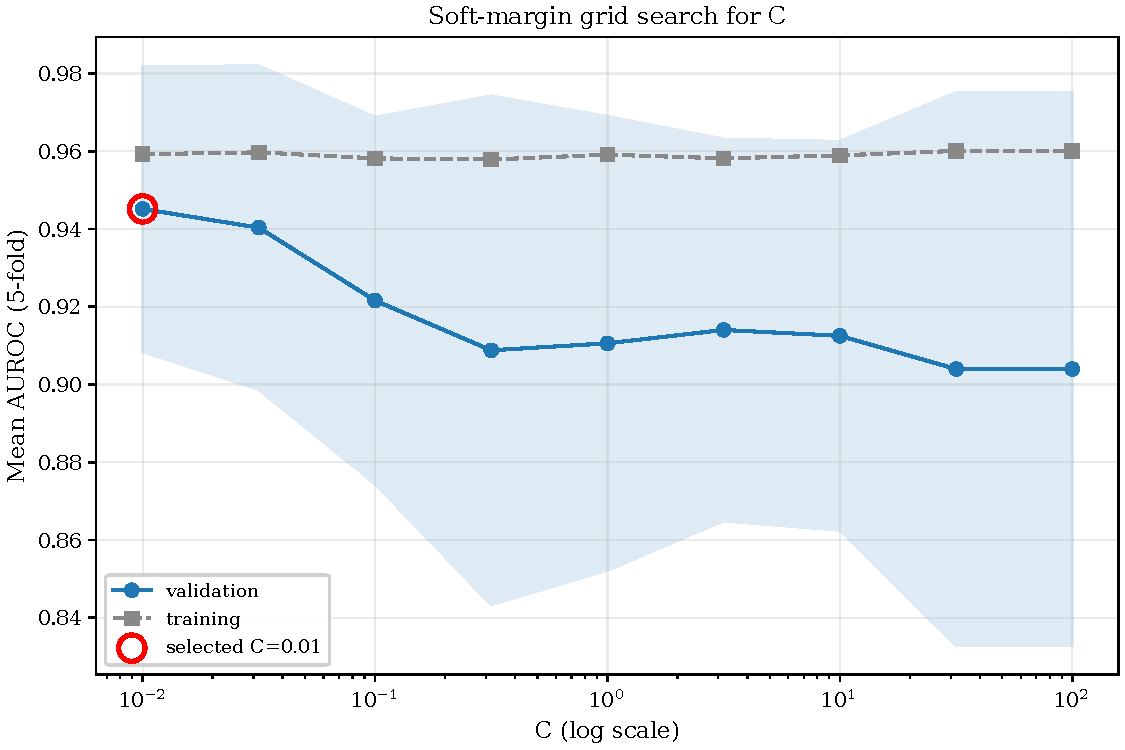
\includegraphics[width=0.8\textwidth]{output/figures/fig_step3_c_grid.pdf}
    \caption{Grid search for the penalty $C$. Mean five-fold validation AUROC
    (with training AUROC for reference) across the $C$ grid; the selected value
    $C=0.01$ is circled. Stronger regularization generalizes best on this
    overlapping data.}
    \label{fig:c-grid}
\end{figure}

\begin{figure}[htbp]
    \centering
    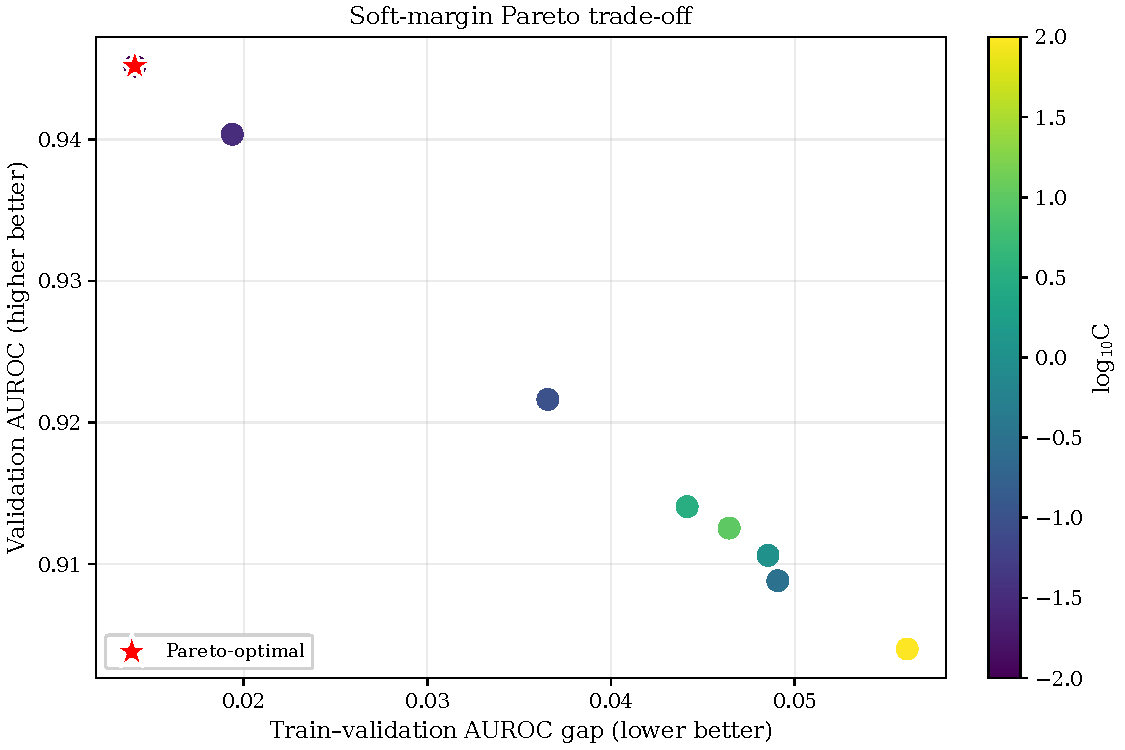
\includegraphics[width=0.8\textwidth]{output/figures/fig_step3_pareto.pdf}
    \caption{The same grid as a Pareto trade-off between mean validation AUROC
    (higher is better) and the train--validation AUROC gap (lower is better).
    Points are colored by $\log_{10}C$; $C=0.01$ (star) is the single
    Pareto-optimal setting.}
    \label{fig:soft-pareto}
\end{figure}

\begin{figure}[htbp]
    \centering
    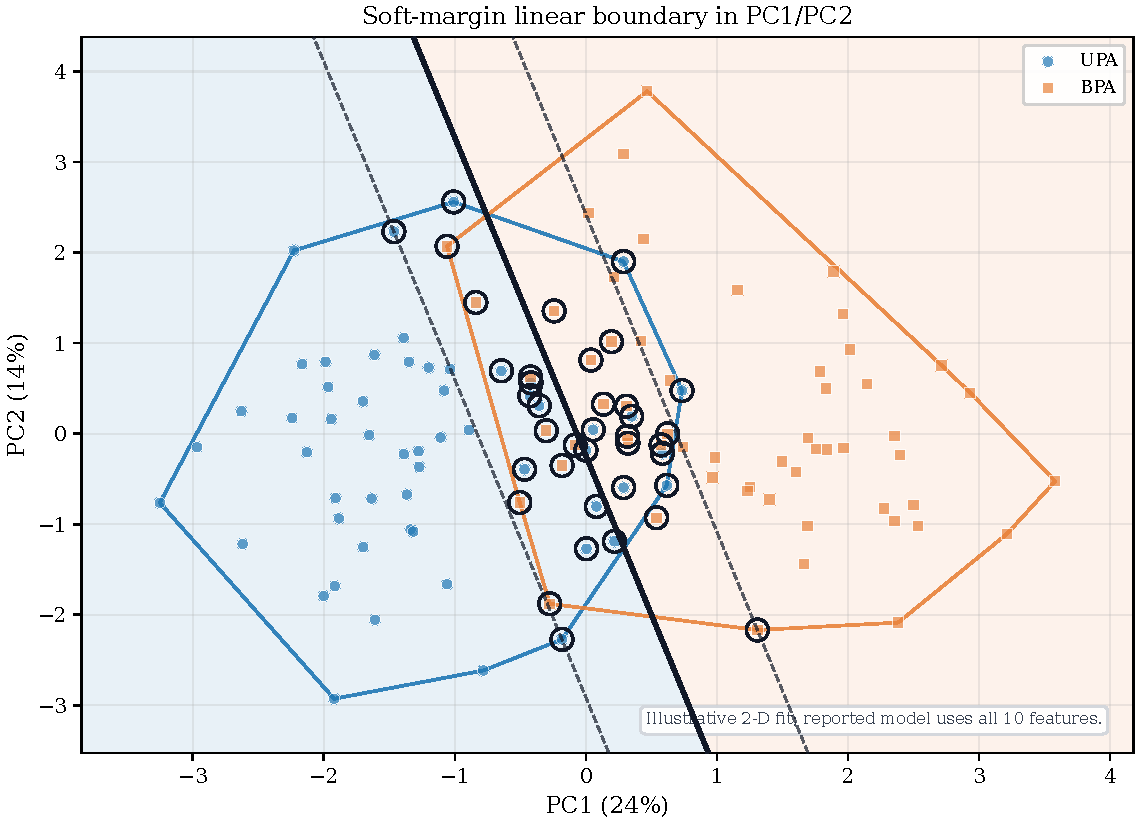
\includegraphics[width=0.72\textwidth]{output/figures/fig_step3c_pc_boundary.pdf}
    \caption{Fitted soft-margin decision boundary in the first two principal
    components, with the $\pm1$ margins and the circled support vectors. The
    boundary is an illustrative two-dimensional fit; the reported model is
    trained on all ten features.}
    \label{fig:soft-boundary}
\end{figure}

\subsection{Solving the Primal Directly: Stochastic Subgradient and Momentum Methods}
\label{sec:sgm}

The dual quadratic program above is solved through \texttt{scikit-learn}'s
LIBSVM-based SVC implementation \cite{chang2011,pedregosa2011}; LIBSVM uses
an SMO-type decomposition strategy related to Platt's algorithm
\cite{platt1998}. The soft-margin \emph{primal} can instead be minimized directly.
Eliminating the slack variables gives hinge losses
$\ell_i(w,b)=\max(0,1-t_i(w^\top x_i+b))$. Dividing the constrained objective
by the positive constant $mC$ does not change its minimizer and gives
\begin{equation}
    P(w,b)=\frac{1}{m}\sum_{i=1}^{m}\ell_i(w,b)
    +\frac{\lambda}{2}\lVert w\rVert^2,
    \qquad \lambda=\frac{1}{mC}.
\end{equation}
This regularized finite sum is a natural target for the stochastic
\emph{subgradient} method (SSG), often grouped under the broader label SGD;
Pegasos is a standard SVM example of this approach \cite{pegasos2011}.
The distinction matters because hinge loss is not differentiable when
$t_i(w^\top x_i+b)=1$. For implementation, let
$\theta=[w^\top,b]^\top$, $z_i=[x_i^\top,1]^\top$, and
$R=\operatorname{diag}(1,\ldots,1,0)$. The zero in $R$ ensures that the
intercept is not regularized. Each step samples one index $k$ uniformly at
random. A valid stochastic subgradient is
\begin{equation}
    g_k(\theta)=\begin{cases}
        \lambda R\theta, & t_k\theta^\top z_k\ge 1,\\[2pt]
        \lambda R\theta-t_k z_k, & t_k\theta^\top z_k<1.
    \end{cases}
\end{equation}
The regularizer is $\lambda$-strongly convex in the weight coordinates
\cite{lec-strongconvex}, while the intercept remains unpenalized. Consequently,
a global strong-convexity guarantee for the full $(w,b)$ vector does not apply
verbatim; the diminishing schedule below is a practical heuristic for this
formulation. The baseline
update is the stochastic subgradient method from the course lecture
\cite{lec-sgm}, $\theta_{k+1}=\theta_k-\eta_k g_k(\theta_k)$. Two momentum variants from the momentum-methods
lecture \cite{lec-momentum} are also evaluated; their classical origins are
Polyak's Heavy Ball method and Nesterov's accelerated method
\cite{polyak1964,nesterov1983}:
\begin{equation}
\begin{aligned}
\text{Heavy Ball:}\quad
    \theta_{k+1}&=\theta_k-\eta_k g_k(\theta_k)+\beta(\theta_k-\theta_{k-1}),\\
\text{Nesterov-style:}\quad
    y_k&=\theta_k+\beta(\theta_k-\theta_{k-1}),\\
    \theta_{k+1}&=y_k-\eta_k g_k(y_k).
\end{aligned}
\end{equation}
The word ``style'' is important: classical Heavy Ball and Nesterov acceleration
theory assumes a smooth gradient, whereas the hinge objective is nonsmooth.
Replacing the gradient by a sampled subgradient gives useful empirical
comparators, but does not inherit the classical accelerated convergence rate.

The optimizer comparison begins only after model selection. The full-data grid
search above selected
\begin{equation}
    \boxed{C=0.01},\qquad
    \lambda=\frac{1}{mC}=\frac{1}{114(0.01)}\approx0.8772.
\end{equation}
Figure~\ref{fig:sgm-convergence} and Table~\ref{tab:sgm-comparison} therefore
optimize the primal for \emph{this one fixed value, $C=0.01$}. They do not
repeat the grid search and do not compare different values of $C$. The
reference optimum for the normalized objective is $P^\star=0.554274$, obtained
by solving the equivalent slack-variable convex quadratic program at
$C=0.01$. Multiplying back by $mC=1.14$ gives the original primal value
$0.6319$, agreeing with the primal--dual solution reported above. For a
controlled comparison, all three algorithms start at zero,
use the same 50,000 sampled observations, and use
$\eta_k=a/[\lambda(k+100)]$. A small common grid
$a\in\{0.25,0.5,1,2\}$ is searched for every method; the momentum methods also
search $\beta\in\{0.3,0.5,0.7,0.9\}$. Within each method, the pair with the
lowest final averaged-iterate objective on a common tuning sequence is
reported. The selected settings are then rerun on ten new, common sampling
sequences to assess optimization robustness. This tuning is only an
optimization diagnostic on the training objective and is not a predictive
performance estimate.

\begin{table}[htbp]
\centering
\caption{Controlled optimizer comparison for the single grid-selected value
$C=0.01$ ($\lambda\approx0.8772$). The
5\% and 1\% columns give the first step at which the best raw iterate reaches
the stated gap relative to $P^\star$; 114 steps correspond to approximately
one epoch. AUROC is in-sample and is shown only as a solution-agreement
diagnostic. Cosine is the similarity of the averaged iterate to the reference
QP solution.}
\label{tab:sgm-comparison}
\scriptsize
\resizebox{\textwidth}{!}{\begin{tabular}{lrrrrrrr}
\toprule
Method & $a$ & $\beta$ & $P(\bar w_K)$ & 5\% steps & 1\% steps & AUROC & Cosine \\
\midrule
SSG & 2.00 & --- & 0.5544 & 96 & 389 & 0.959 & 1.000 \\
Heavy Ball & 0.25 & 0.9 & 0.5544 & 150 & 391 & 0.959 & 1.000 \\
Nesterov-style & 2.00 & 0.3 & 0.5544 & 98 & 389 & 0.959 & 1.000 \\
\bottomrule
\end{tabular}
}
\end{table}

Because a single sampled-observation sequence can make a stochastic optimizer
look unusually favorable, Table~\ref{tab:sgm-robustness} repeats the already
selected optimizer settings on ten new common sampling sequences. Medians and
interquartile ranges (IQRs) are descriptive optimization diagnostics.

\begin{table}[htbp]
\centering
\caption{Robustness over ten new common sampling sequences at the single fixed
value $C=0.01$. Hyperparameters were selected on the separate seed-2026
sequence.}
\label{tab:sgm-robustness}
\scriptsize
\resizebox{\textwidth}{!}{\begin{tabular}{lrrr}
\toprule
Method & Final gap, median [IQR] & 5\% steps, median [IQR] & 1\% steps, median [IQR] \\
\midrule
SSG & 1.45e-04 [1.30e-04, 1.82e-04] & 41 [34, 48] & 260 [186, 353] \\
Heavy Ball & 1.49e-04 [1.42e-04, 1.91e-04] & 60 [35, 73] & 519 [296, 558] \\
Nesterov-style & 1.54e-04 [1.44e-04, 1.99e-04] & 39 [29, 50] & 356 [256, 510] \\
\bottomrule
\end{tabular}
}
\end{table}

\begin{figure}[htbp]
    \centering
    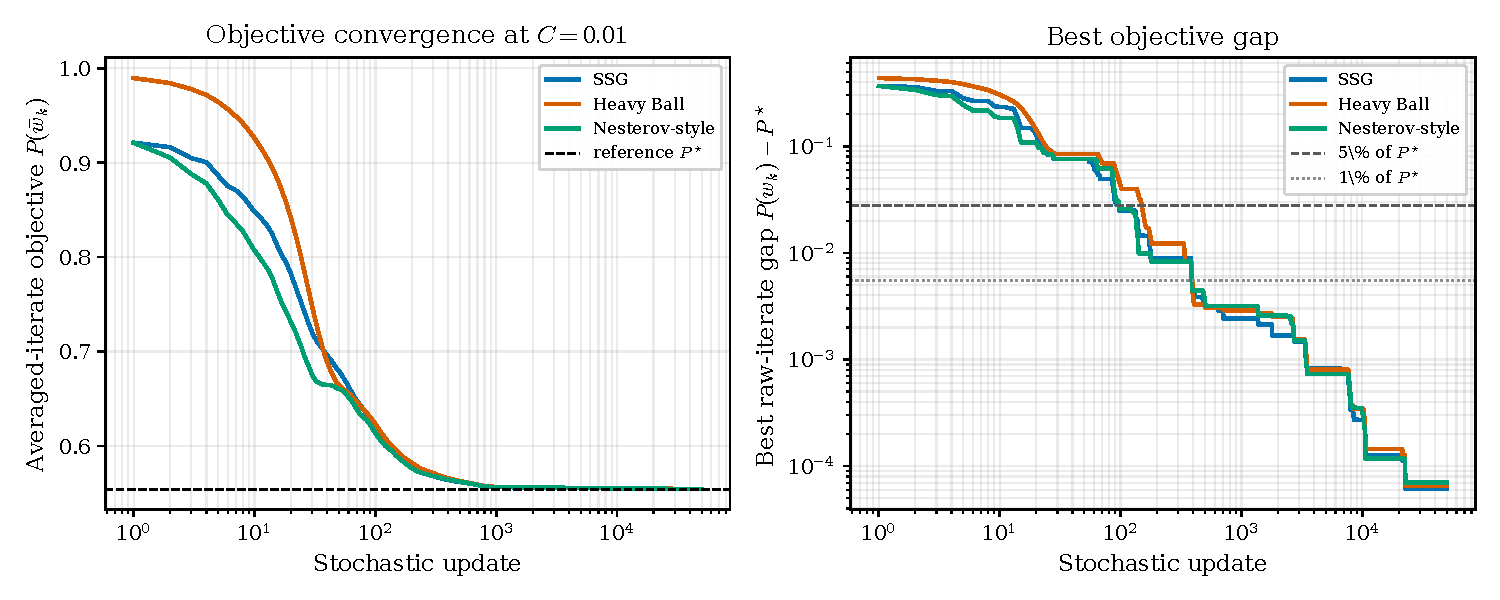
\includegraphics[width=\textwidth]{output/figures/primal_optimizer_comparison.pdf}
    \caption{Stochastic primal optimization for the fixed selected value
    $C=0.01$ ($\lambda\approx0.8772$), under a shared data sequence and
    iteration budget. Left: objective values of the running averaged iterates.
    Right: best-so-far raw-iterate optimality gaps. All three methods approach
    the same reference optimum, but momentum does not accelerate this
    nonsmooth stochastic problem under the tested settings.}
    \label{fig:sgm-convergence}
\end{figure}

The illustrative seed-2026 comparison does not show a meaningful momentum advantage. SSG reaches the
5\% gap in 96 updates (0.84 epochs) and the 1\% gap in 389 updates (3.41
epochs). Heavy Ball reaches the two thresholds in 150 and 391 updates, while
the Nesterov-style method requires 98 and 389 updates. All averaged iterates
have objective approximately $0.5544$, in-sample AUROC approximately $0.959$,
and cosine similarity above $0.9998$ to the reference solution. Thus the
methods converge to essentially the same fixed-$C$ classifier, while plain SSG
is the simplest and at least as fast under this controlled run. This negative acceleration result
is plausible: strong convexity does not remove the hinge kink, sampled
subgradients remain noisy near the optimum, and the smooth-gradient Heavy Ball
and Nesterov rate guarantees do not apply. Running averages stabilize all
three methods. Across the ten new sequences, median final gaps are
$1.45\times10^{-4}$ for SSG, $1.49\times10^{-4}$ for Heavy Ball, and
$1.54\times10^{-4}$ for Nesterov-style. Median steps to the 1\% threshold are
260, 519, and 356, respectively. The sequence-to-sequence variation reinforces
the conclusion: none of the momentum variants provides a robust acceleration
advantage under this fixed budget and tuning protocol.

\section{Kernel Trick: RBF Soft-Margin SVM}
\label{sec:kernel-rbf}

\subsection{From a Linear Boundary to a Kernel Boundary}

The strong linear soft-margin result does not prove that a nonlinear boundary
is unnecessary; it only establishes a competitive baseline. The kernel trick
tests nonlinear structure without explicitly constructing a potentially
high-dimensional feature vector. Let
$\varphi(x)$ map an observation into a feature space $\mathcal{H}$. The
soft-margin primal in that space is
\begin{equation}
\begin{aligned}
\min_{w,b,\xi}\quad
&\frac12\lVert w\rVert_{\mathcal H}^2+C\sum_{i=1}^{m}\xi_i\\
\text{subject to}\quad
&t_i(\langle w,\varphi(x_i)\rangle_{\mathcal H}+b)
\geq1-\xi_i,\qquad \xi_i\geq0.
\end{aligned}
\end{equation}
The corresponding dual depends on transformed observations only through inner
products:
\begin{equation}
\begin{aligned}
\max_{\alpha}\quad
&\sum_i\alpha_i-
\frac12\sum_i\sum_j\alpha_i\alpha_jt_it_jK(x_i,x_j)\\
\text{subject to}\quad
&0\leq\alpha_i\leq C,\qquad \sum_i\alpha_it_i=0,
\end{aligned}
\end{equation}
where
$K(x_i,x_j)=\langle\varphi(x_i),\varphi(x_j)\rangle_{\mathcal H}$.
The fitted score is
\begin{equation}
    f(x)=\sum_{i\in\mathcal S}\alpha_i t_iK(x_i,x)+b,
\end{equation}
so only the support-vector set $\mathcal S$ is needed at prediction time.
Kernelization does not replace the soft margin: $C$ still bounds each dual
multiplier and controls the penalty for overlap.

This analysis uses the radial basis function (RBF) kernel
\begin{equation}
    K(x_i,x_j)=\exp[-\gamma\lVert x_i-x_j\rVert_2^2].
\end{equation}
Small $\gamma$ produces a smooth, slowly varying decision surface and tends
toward linear-like behavior over a limited data region. Large $\gamma$ makes
each observation influential only in a narrow neighborhood, allowing a highly
curved boundary that can memorize a small training cohort. Therefore $C$ and
$\gamma$ must be tuned jointly.

\subsection{Validity of the RBF Kernel: Positive Semi-Definiteness and
Feature Map}
\label{sec:rbf-psd}

Everything above presumes that some feature map $\varphi$ exists with
$K(x,y)=\langle\varphi(x),\varphi(y)\rangle_{\mathcal H}$. That is not
automatic: an arbitrary similarity function need not be an inner product in
any space, and if it is not, the dual loses concavity and the optimization
guarantees of Section~\ref{sec:slater} no longer apply. This subsection
establishes the two properties that license the RBF kernel.

A symmetric kernel $K$ is \emph{positive semi-definite} (PSD) if for every
finite set $x_1,\ldots,x_m$ the Gram matrix $G_{ij}=K(x_i,x_j)$ satisfies
$c^\top Gc\geq0$ for all $c\in\mathbb{R}^m$. Four standard closure rules are
used \cite{boyd2004,lec-statlearn}: if $K_1,K_2$ are PSD then (K1) $\lambda_1K_1+\lambda_2K_2$
is PSD for $\lambda_1,\lambda_2\geq0$; (K2) the product $K_1K_2$ is PSD, by the
Schur product theorem; (K3) $K(x,y)=f(x)f(y)$ is PSD for any real $f$; and
(K4) a pointwise limit of PSD kernels is PSD.

\paragraph{The RBF kernel is PSD.}
The linear kernel is PSD because
\begin{equation}
    c^\top Gc=\sum_{i}\sum_{j}c_ic_j\,x_i^\top x_j
    =\Bigl\lVert\sum_{i}c_ix_i\Bigr\rVert_2^2\geq0,
\end{equation}
so $(x^\top y)^k$ is PSD for every integer $k\geq0$ by repeated application of
(K2). The exponential series has non-negative coefficients, hence
\begin{equation}
    \exp\bigl[2\gamma\,x^\top y\bigr]
    =\sum_{k=0}^{\infty}\frac{(2\gamma)^k}{k!}\,(x^\top y)^k
\end{equation}
is a limit of non-negative combinations of PSD kernels and is PSD by (K1) and
(K4). Expanding the squared norm as
$\lVert x-y\rVert_2^2=\lVert x\rVert_2^2-2x^\top y+\lVert y\rVert_2^2$
factors the RBF kernel into
\begin{equation}
    \exp\bigl[-\gamma\lVert x-y\rVert_2^2\bigr]
    =\underbrace{e^{-\gamma\lVert x\rVert_2^2}
      e^{-\gamma\lVert y\rVert_2^2}}_{\text{PSD by (K3)}}
    \cdot
    \underbrace{\exp\bigl[2\gamma\,x^\top y\bigr]}_{\text{PSD}},
\end{equation}
which is PSD by (K2). The Gram matrix is therefore PSD for any dataset and any
$\gamma>0$.

\paragraph{An explicit feature map.}
The same expansion produces $\varphi$ directly. Writing the multinomial
expansion of $(x^\top y)^k$ over multi-indices
$\nu\in\mathbb{N}_0^{p}$, with $\lvert\nu\rvert=\sum_j\nu_j$,
$\nu!=\prod_j\nu_j!$ and $x^\nu=\prod_jx_j^{\nu_j}$, gives
\begin{equation}
    \exp\bigl[2\gamma\,x^\top y\bigr]
    =\sum_{\nu\in\mathbb{N}_0^{p}}
      \frac{(2\gamma)^{\lvert\nu\rvert}}{\nu!}\,x^\nu y^\nu .
\end{equation}
Reinstating the two Gaussian factors and splitting each term symmetrically
yields $K(x,y)=\langle\varphi(x),\varphi(y)\rangle$ with components
\begin{equation}
    \varphi_\nu(x)=e^{-\gamma\lVert x\rVert_2^2}
    \sqrt{\frac{(2\gamma)^{\lvert\nu\rvert}}{\nu!}}\;x^\nu,
    \qquad \nu\in\mathbb{N}_0^{p}.
\end{equation}
The index set is all multi-indices, so $\mathcal H$ is
infinite-dimensional: $\varphi$ contains every monomial in the $p$ features,
damped by $e^{-\gamma\lVert x\rVert_2^2}$ and weighted so the series converges.

\paragraph{Consequences.}
Three points follow. First, the exact feature map is infinite-dimensional and
is therefore not represented as a finite explicit feature vector in this
analysis; the scalar $K(x_i,x_j)$ instead evaluates the required inner product
directly. Second, PSD of the Gram matrix makes the dual objective concave, so
every local optimum is globally optimal and there are no spurious local
maxima. PSD alone does not require the optimal dual coefficients to be unique.
Third, the primal in $\mathcal H$ is convex with affine constraints and admits
the strictly feasible point
$(w,b,\xi)=(0,0,2\mathbf{1})$, so Slater's condition holds exactly as in
Section~\ref{sec:slater}. Although $\mathcal H$ is infinite-dimensional, the
representer theorem restricts an optimum to the finite span of the training
feature vectors, which connects this statement to the finite Gram-matrix dual;
the primal--dual gap of $2.2\times10^{-11}$ reported
for the fitted RBF model is therefore a meaningful check that the solver
reached a global optimum.

\subsection{Joint Grid Search and Nested Validation}

The RBF analysis uses the same log transformation, median imputation,
standardization, stratified folds, and random seed as the linear analysis. The
joint grid contains nine values of $C$ from $0.01$ to $100.00$ and nine values
of $\gamma$ from $1.00\times10^{-3}$ to $10.00$, both at half-logarithmic
spacing. Thus each inner search evaluates 81 parameter pairs by mean AUROC.

In every outer fold, preprocessing and the complete 81-point grid search are
fitted using only the outer training data. Table~\ref{tab:rbf-nested} shows
that the selected pairs vary substantially across folds. This instability is
itself relevant: with only 114 observations, the apparently best nonlinear
scale depends on which observations enter the training set.

\begin{table}[H]
\centering
\caption{Nested cross-validation for joint RBF tuning. AUROC values and parameter displays use two decimals or two-decimal scientific notation.}
\label{tab:rbf-nested}
\small
\begin{tabular}{rrrrrr}
\toprule
Fold & $C$ & $\gamma$ & Inner train & Inner validation & Outer AUROC \\
\midrule
1 & 3.16 & 1.00e-03 & 0.97 & 0.95 & 0.92 \\
2 & 10.00 & 1.00e-03 & 0.96 & 0.96 & 0.94 \\
3 & 0.32 & 0.03 & 0.96 & 0.94 & 0.98 \\
4 & 1.00 & 3.16e-03 & 0.95 & 0.92 & 0.98 \\
5 & 0.01 & 1.00e-03 & 0.97 & 0.96 & 0.88 \\
Mean & --- & --- & 0.962 & 0.946 & 0.942 \\
\bottomrule
\end{tabular}

\end{table}

The full-data grid search selected $C=0.01$ and
$\gamma=1.00\times10^{-3}$. Here $\gamma$ is an inverse squared-bandwidth
parameter: smaller values give wider, smoother kernels. This $\gamma$ is the lower boundary of the
prespecified grid, indicating that the validation criterion favors the
smoothest candidate rather than a strongly nonlinear boundary. At the
selected pair, mean training AUROC is $0.96$ and mean validation AUROC is
$0.95$, a gap of only $0.01$. The induced-feature-space primal and dual
objectives both round to $1.12$, with full-precision duality gap
$2.23\times10^{-11}$.

\begin{table}[H]
\centering
\caption{Full-data RBF model-selection and optimization audit.}
\label{tab:rbf-summary}
\begin{tabular}{lr}
\toprule
Quantity & Value \\
\midrule
Selected $C$ & 0.01 \\
Selected $\gamma$ & 1.00e-03 \\
Mean training AUROC & 0.96 \\
Mean validation AUROC & 0.95 \\
Train--validation gap & 0.01 \\
Largest gap anywhere on grid & 0.46 \\
Mean nested outer AUROC & 0.94 \\
Support vectors & 113 \\
Observations with $\xi_i>0$ & 111 \\
Primal objective & 1.12 \\
Dual objective & 1.12 \\
\bottomrule
\end{tabular}

\end{table}

\subsection{Overfitting Diagnostic}

The selected RBF model is not strongly overfit, but the grid contains a clear
demonstration of the risk. Figure~\ref{fig:rbf-grid} compares validation AUROC
with the train--validation gap. At $C=0.01$ and $\gamma=10.00$, training AUROC
is $1.00$ while validation AUROC falls to $0.54$, giving a gap of $0.46$.
Across all values of $C$ at $\gamma=10.00$, training AUROC remains $1.00$ but
validation AUROC is only $0.54$--$0.59$. The high-$\gamma$ kernel has therefore
memorized the training folds without learning a stable decision rule.

\begin{figure}[H]
    \centering
    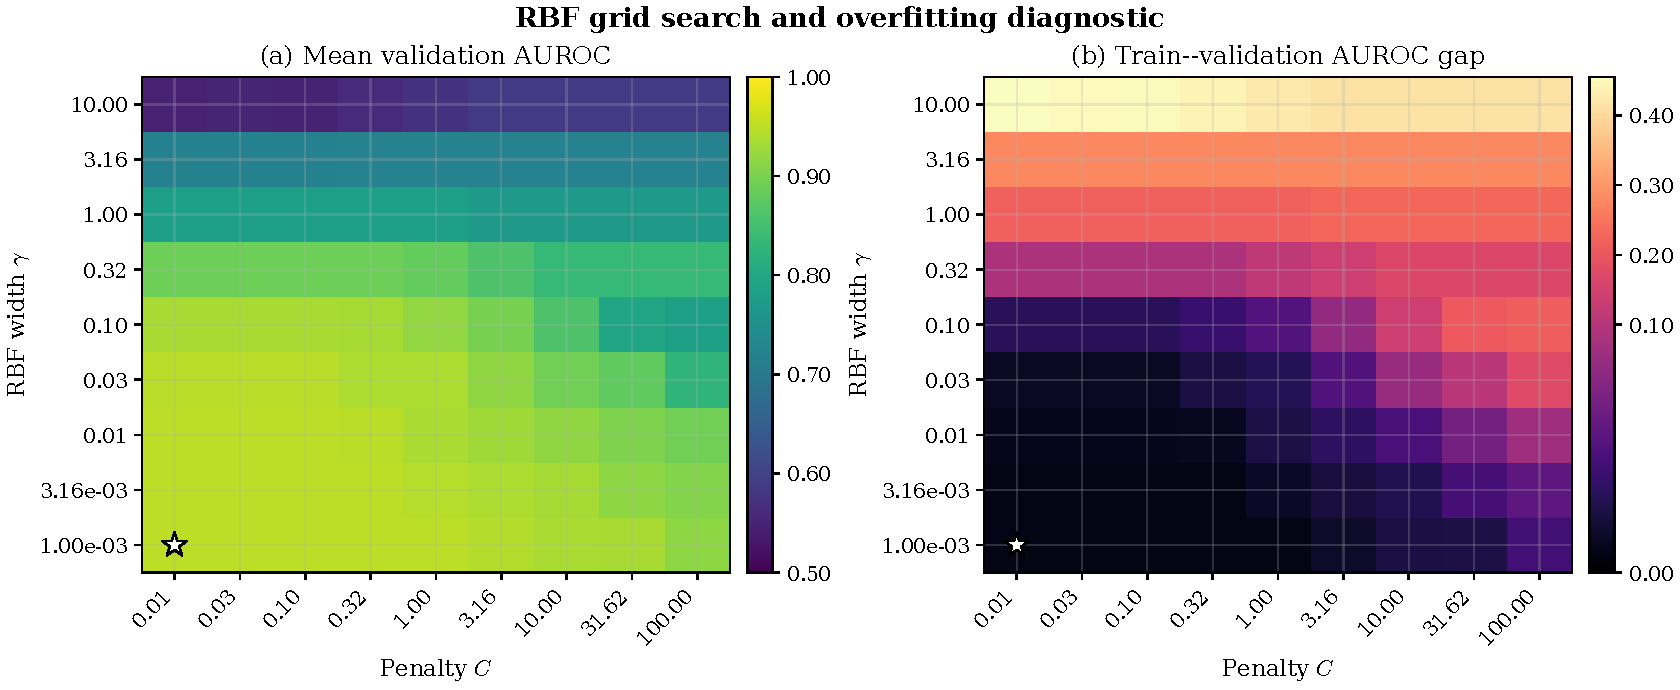
\includegraphics[width=0.98\textwidth]{output/figures/rbf_kernel_grid_heatmaps.pdf}
    \caption{Joint RBF grid search. Panel (a) shows mean validation AUROC. Panel (b) shows mean training AUROC minus mean validation AUROC; large positive values indicate overfitting. The white star marks the selected full-data pair $C=0.01$, $\gamma=1.00\times10^{-3}$.}
    \label{fig:rbf-grid}
\end{figure}

This result illustrates why training performance cannot be used to choose a
kernel. A nonlinear model can achieve perfect training ranking precisely where
its held-out ranking is close to chance. Nested validation, the
train--validation gap, and the position of the selected point on the grid must
be interpreted together.

Figure~\ref{fig:rbf-boundary} shows the RBF decision surface in the same
principal-component projection as the linear boundary of
Figure~\ref{fig:soft-boundary}. The kernel lets the boundary curve, but the two
convex hulls still overlap: the added flexibility bends the surface around
individual points without producing a clean separation in this illustrative
two-dimensional fit. This picture motivates the comparison but does not decide
which model generalizes better; that conclusion comes from the untouched outer
folds below.

\begin{figure}[htbp]
    \centering
    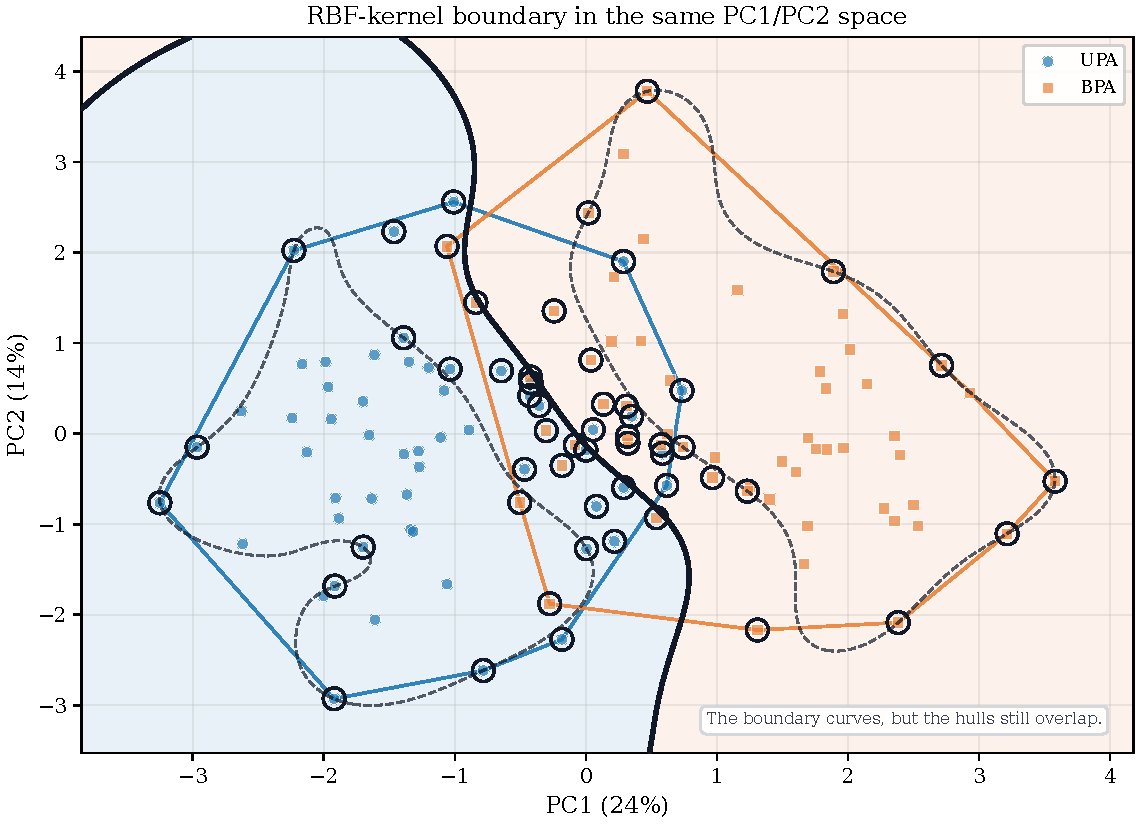
\includegraphics[width=0.72\textwidth]{output/figures/fig_step4_rbf_pc_boundary.pdf}
    \caption{RBF-kernel decision boundary in the first two principal components,
    to be compared with the straight linear boundary of
    Figure~\ref{fig:soft-boundary}. The boundary curves but the subtype hulls
    still overlap. Illustrative two-dimensional fit at a moderate $\gamma$; the
    tuned model selected a much smoother $\gamma$.}
    \label{fig:rbf-boundary}
\end{figure}

\subsection{Pareto Frontier of Validation Performance and Overfitting}

A Pareto analysis makes this trade-off explicit. The two objectives are to
maximize mean validation AUROC and minimize the train--validation AUROC gap.
Grid setting A dominates setting B when A has validation AUROC no smaller and
an overfitting gap no larger, with at least one strict improvement. A setting
is Pareto-optimal when no other setting dominates it. The hyperparameters
$C$ and $\gamma$ identify the grid settings; they are not themselves the two
Pareto objectives.

Figure~\ref{fig:pareto-frontier} plots every evaluated setting. For the linear
soft-margin grid, the frontier collapses to one point:
\begin{equation}
    C=0.01,\qquad
    \operatorname{AUROC}_{\mathrm{val}}=0.9452,\qquad
    \operatorname{gap}=0.0141.
\end{equation}
Every other tested linear value of $C$ has both a lower validation AUROC and a
larger train--validation gap.

The RBF grid has a four-setting Pareto plateau. All four use
$\gamma=0.00316$ and
\begin{equation}
    C\in\{0.01,0.0316,0.10,0.3162\},
\end{equation}
with validation AUROC $0.9511$ and gap $0.0083$ to stored precision. Because
their two Pareto outcomes are indistinguishable, the smallest value $C=0.01$
is the natural simplicity tie-break. The ordinary grid search reported
$\gamma=0.001$ because it has the same maximum validation AUROC and appears
first among tied scores; the Pareto diagnostic instead identifies
$\gamma=0.00316$ because its train--validation gap is smaller by approximately
$2.06\times10^{-6}$. This difference is far below the fold-to-fold standard
deviations. It is numerically negligible and does not
constitute evidence of a meaningful nonlinear advantage.

\begin{figure}[H]
    \centering
    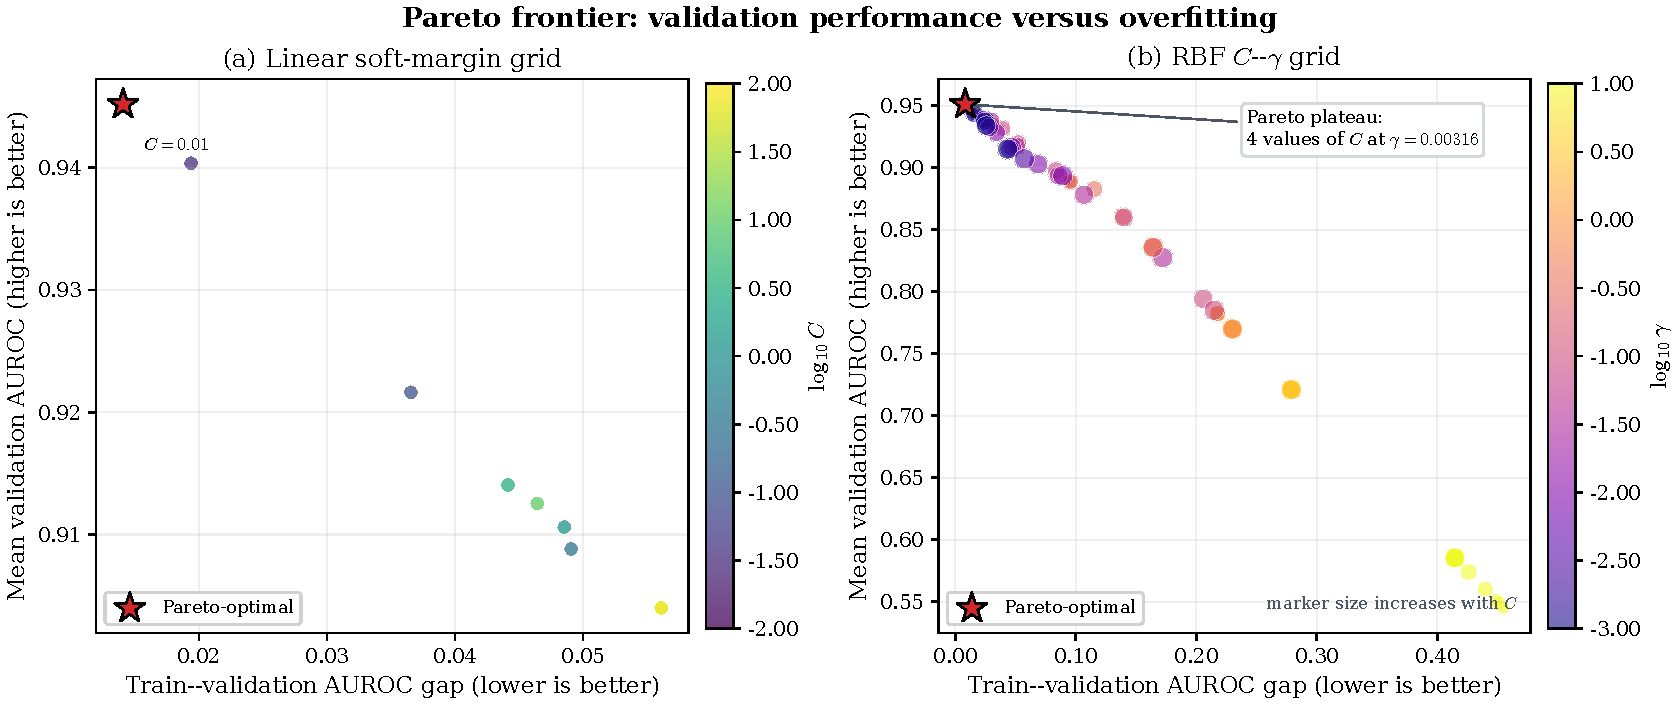
\includegraphics[width=0.98\textwidth]{output/figures/svm_grid_pareto_frontier.pdf}
    \caption{Pareto analysis of the linear and RBF tuning grids. The horizontal axis is the train--validation AUROC gap, so smaller values are preferred; the vertical axis is mean validation AUROC, so larger values are preferred. Red stars mark non-dominated settings. In panel (a), color represents $\log_{10}C$. In panel (b), color represents $\log_{10}\gamma$ and marker size increases with $C$.}
    \label{fig:pareto-frontier}
\end{figure}

This frontier is a tuning diagnostic computed from the cross-validated grid;
it is not an independent performance estimate. Selecting a point from the
frontier and then quoting the same validation folds would be optimistic. The
final linear-versus-RBF conclusion therefore continues to use the untouched
nested outer folds in the next subsection.

\subsection{Comparison with the Linear Soft-Margin Model}
\label{sec:kernel-comparison}

For the prespecified seed-zero split, the comparison uses mean outer-fold
AUROC because each outer fold is untouched by its corresponding parameter search. The linear model achieves
$0.95\pm0.04$, whereas the RBF model achieves $0.94\pm0.04$. The RBF-minus-linear
difference in mean outer AUROC is $-3.17\times10^{-3}$, so there is no observed
improvement from the kernel. The RBF accuracy is $0.82$, sensitivity is
$0.73$, and specificity is $0.91$, compared with approximately $0.86$ for all
three quantities under the linear model.

\begin{table}[H]
\centering
\caption{Seed-zero nested cross-validation comparison of linear and RBF soft-margin SVMs. SD is the sample standard deviation across five outer folds ($\mathrm{ddof}=1$). Mean outer-fold AUROC avoids cross-fold score-scale artifacts; repeated-seed results provide the headline stability comparison.}
\label{tab:kernel-comparison}
\small
\begin{tabular}{lrrrrrr}
\toprule
Model & Mean outer AUC & SD & Pooled AUC & Accuracy & Sensitivity & Specificity \\
\midrule
Linear soft margin & 0.95 & 0.04 & 0.95 & 0.86 & 0.86 & 0.86 \\
RBF kernel & 0.94 & 0.04 & 0.85 & 0.82 & 0.73 & 0.91 \\
\bottomrule
\end{tabular}

\end{table}

The pooled RBF AUROC is shown for completeness but is not the primary estimate.
Different outer folds selected different $(C,\gamma)$ pairs, so their raw
decision scores have different scales and pooling can alter cross-fold ranks.
The mean of the five independently evaluated outer-fold AUROCs avoids this
scale-comparability problem. This warning concerns rank pooling for AUROC;
accuracy, sensitivity, and specificity use each classifier's invariant
decision-sign threshold and are not invalidated by positive score rescaling.
Figure~\ref{fig:linear-rbf-roc} therefore averages
fold-specific ROC curves on a common false-positive-rate grid.

\begin{figure}[H]
    \centering
    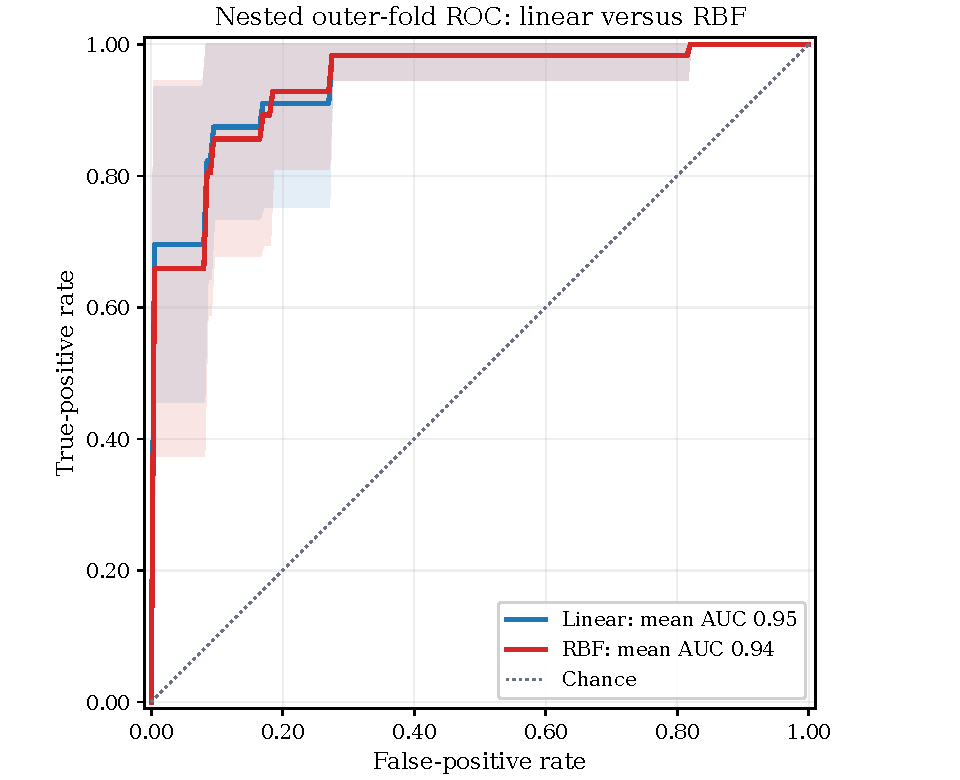
\includegraphics[width=0.70\textwidth]{output/figures/linear_vs_rbf_nested_roc.pdf}
    \caption{Mean nested outer-fold ROC curves for the linear and RBF soft-margin models. Shaded bands show one standard deviation across the five outer folds.}
    \label{fig:linear-rbf-roc}
\end{figure}

This seed-zero result is illustrative; the twenty-seed analysis in
Section~\ref{sec:stat-comparison} is the more stable headline comparison. The
present data do not support retaining the RBF kernel. It adds a second
hyperparameter, produces unstable fold-specific choices, selects the smoothest
available $\gamma$ on the full dataset, and does not improve the mean nested
outer-fold AUROC.
With only 114 synthetic observations, a flexible high-$\gamma$ boundary has a
substantial overfitting risk. The linear soft-margin model is therefore the
preferred specification unless a larger independent dataset demonstrates a
reproducible nonlinear improvement.

The numerical values of $C$ should not be compared literally across the
linear and RBF models: kernel normalization changes the geometry and effective
regularization scale. The comparison is between separately tuned model
families using untouched outer folds, not between equal-valued penalties.

The complete grid, nested predictions, support-vector audit, primal--dual
checks, comparison table, and figures are generated by
\path{scripts/kernel_rbf_svm.py} and written under \path{output/csv/} and
\path{output/figures/}.

\section{Integrated Results Summary}

The feasible ten-row calculation in Appendix~\ref{app:worked-examples} is an
algebraic illustration only. The report's feasibility conclusion is based on
the complete standardized dataset and all five cross-validation training
folds. Every full analysis problem was declared infeasible by the HiGHS
linear-programming solver, as summarized earlier in
Table~\ref{tab:feasibility}.

These outcomes show that the UPA and BPA observations overlap in the selected
ten-dimensional linear feature space. This is a property of the data geometry
rather than a failure of the quadratic optimizer.
Section~\ref{sec:full-certificate} strengthens the solver status with an
explicit Farkas certificate: a nonnegative vector satisfies
$U^\top\lambda\approx0$ and $\mathbf{1}^\top\lambda=1$, proving that the
standardized class convex hulls intersect. Consequently, the hard-margin
primal cannot be fitted and no hard-margin ROC exists.

The soft-margin model converts this empty feasible set into a feasible convex
program by allowing penalized slack. Grid search selected $C=0.01$. Its mean
five-fold validation AUROC was $0.95$, while seed-zero nested cross-validation produced
pooled out-of-fold AUROC $0.95$, accuracy $0.86$, sensitivity $0.86$, and specificity
$0.86$. The full-data primal and dual objectives both round to $0.63$, with a
full-precision duality gap of $4.85\times10^{-10}$. These soft-margin results
are kept distinct from the infeasible hard-margin formulation.

On the illustrative seed-zero partition, the RBF experiment did not improve
mean outer-fold AUROC ($0.94\pm0.04$ versus $0.95\pm0.04$ for linear). Across
twenty split seeds, however, both model families average approximately $0.94$
(linear $0.9401$, RBF $0.9399$), with no stable winner. The selected full-data pair was $C=0.01$ and
$\gamma=1.00\times10^{-3}$, with $\gamma$ at the smoothest boundary of the
grid. High-$\gamma$ combinations achieved training AUROC $1.00$ while falling
as low as validation AUROC $0.54$, demonstrating substantial overfitting. The
Pareto audit retained one linear setting and a four-setting RBF plateau when
validation AUROC was maximized jointly with minimization of the
train--validation gap; it did not change the parsimony-based preference for the
linear model after the repeated nested comparison found an effective tie.

\section{Discussion and Limitations}

The derivative analysis confirms that the hard-margin primal is a simple convex quadratic program: its objective has gradient $[w^\top,0]^\top$ and positive-semidefinite Hessian $\operatorname{diag}(I_p,0)$, while each constraint is affine. These properties make any feasible instance globally tractable. They do not, however, guarantee that a feasible point exists.

The feasible teaching subset does not contradict the full-data result: feasibility is lost when the remaining 104 margin constraints are added.

The negative hard-margin feasibility result is substantively consistent with
the application. Clinical measurements from UPA and BPA patients can overlap
because of biological heterogeneity, measurement variation, and incomplete
diagnostic information. A hard-margin linear model assumes away this overlap.
The soft-margin formulation is therefore not a workaround for a failed
solver; it is a different, explicitly stated optimization model whose slack
variables quantify the overlap.

AUROC evaluates ranking over all thresholds; it does not establish calibrated
probabilities or a clinically acceptable operating point. The threshold-zero
sensitivity and specificity are descriptive for these fitted margins and were
not chosen from a decision-analytic cost function. A real subtype workflow
would also need comparison with definitive clinical procedures such as adrenal
venous sampling, prospective calibration, and external validation. None of
those claims can be made from this synthetic cohort.

The selected value $C=0.01$ lies at the lower end of the prespecified grid.
This indicates that stronger regularization was preferred to aggressively
penalizing every violation. The neighboring value $C=0.03$ produced a similar
mean validation AUROC, so the exact numerical optimum should not be treated as
a universal clinical constant. It is specific to this feature scaling,
candidate grid, synthetic cohort, folds, and selection metric. Nested
cross-validation reduces selection optimism but does not replace external
validation.

Because both primary selections touched lower grid boundaries, an explicitly
post-selection sensitivity analysis extended $C$ to $10^{-4}$ and $\gamma$ to
$10^{-5}$ on the full-data five-fold validation split. Table~\ref{tab:boundary-sensitivity}
shows that the validation criterion continues toward an even more strongly
regularized, smoother limit: four linear $C$ values from $10^{-4}$ through
$3.16\times10^{-3}$ tie at AUROC $0.950$, and the extended RBF maximum is
attained on a three-setting plateau whose smallest setting is
$C=10^{-4},\gamma=10^{-5}$ (AUROC $0.953$). This exploratory audit does not
replace or retroactively retune the prespecified nested-CV protocol. Instead,
it shows that neither hyperparameter is precisely identified and that the
data favor an almost linear, heavily regularized ranking. The tiny validation
differences are well below fold-level uncertainty.

\begin{table}[htbp]
\centering
\caption{Post-selection lower-bound sensitivity check. The primary choices
remain the prespecified-grid results used in nested validation.}
\label{tab:boundary-sensitivity}
\scriptsize
\resizebox{\textwidth}{!}{\begin{tabular}{llll}
\toprule
Model & Primary grid choice & Extended-grid result & Interpretation \\
\midrule
Linear & $C=0.01$ & best AUROC 0.950; $C\in[10^{-4},3.16\!\times\!10^{-3}]$ tied & lower-$C$ plateau \\
RBF & $C=0.01,\ \gamma=10^{-3}$ & best AUROC 0.953; 3-setting tie; smallest $C=10^{-4},\ \gamma=10^{-5}$ & smoother-limit solution \\
\bottomrule
\end{tabular}
}
\end{table}

The RBF comparison reinforces this limitation. Jointly searching 81
$(C,\gamma)$ combinations increases the opportunity to select noise, and the
preferred pair varied substantially between outer folds. The nested analysis
found no performance gain, while the high-$\gamma$ region produced perfect
training AUROC and near-chance validation. Model complexity should therefore
not be justified by training fit.

\subsection{Robustness of the Linear--RBF Comparison}
\label{sec:stat-comparison}

The primary comparison above uses mean AUROC across untouched outer folds.
Two additional diagnostics explain why the conclusion is deliberately modest:
the evidence supports choosing the simpler linear model, but it does not show
that the linear model has intrinsically superior discrimination.

\paragraph{Pooled out-of-fold discrimination.}
On the pooled out-of-fold decision scores, the linear soft-margin AUROC
($0.947$) exceeds the RBF AUROC ($0.851$). This number is not a valid primary
head-to-head estimate for the score-scale reason established in
Section~\ref{sec:kernel-comparison}. The pooled gap and its naive DeLong or
patient-bootstrap significance tests are therefore not used to choose the
model, and no formal inference is attached to this scale-sensitive pooled
calculation.

\paragraph{Mean outer-fold discrimination and seed robustness.}
The fairer comparison computes AUROC within each untouched outer fold and then
averages the five values. Repeating the full nested procedure under twenty
fold-assignment seeds, the linear and RBF estimates track each other closely
(Figure~\ref{fig:seed-robustness}). The mean difference is $+0.0002$, the
descriptive $95\%$ interval across seeds is $[-0.022,\,+0.017]$, and the linear
model equals or exceeds the RBF model in twelve of twenty runs. These repeated
splits reuse the same 114 observations and are therefore a stability analysis,
not twenty independent experiments; the displayed empirical quantiles have no
frequentist coverage interpretation. They show that the direction of the tiny
gap depends on the split and provide no stable discrimination advantage for
either model.

\paragraph{Interpretation.}
The diagnostics answer different questions. The pooled calculation exposes a
cross-fold score-scaling problem; the repeated nested analysis shows that the
proper fold-wise comparison is essentially tied. Because nonlinear flexibility
does not deliver a stable outer-fold gain, the linear model is preferred on
grounds of parsimony, fewer tuning degrees of freedom, and a directly
inspectable standardized-space score.

\begin{figure}[H]
    \centering
    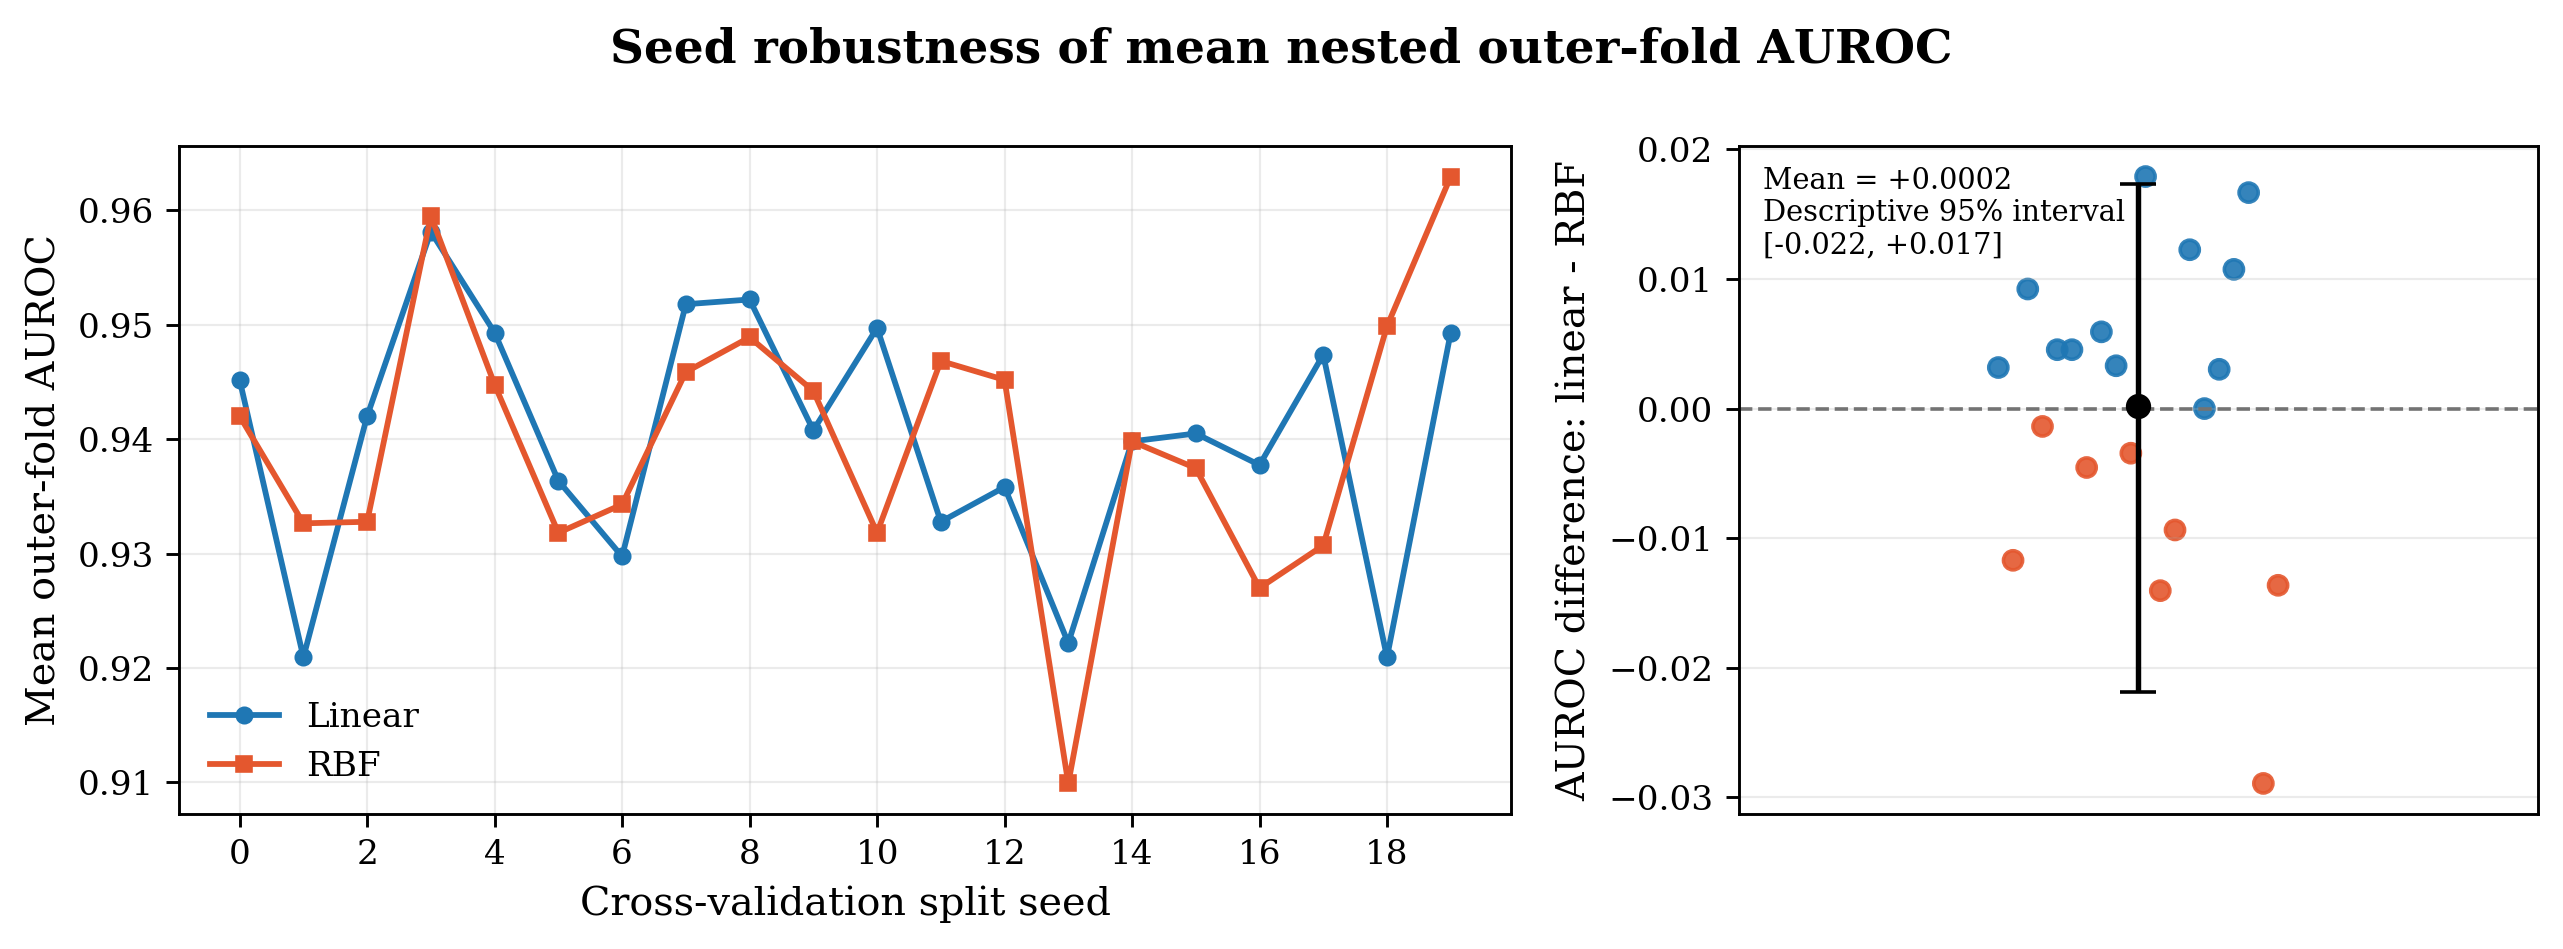
\includegraphics[width=\textwidth]{output/figures/fig_stat_seed_robustness.png}
    \caption{Seed-robustness of the fairer mean outer-fold AUROC. Panel (a):
    linear and RBF values across twenty fold-assignment seeds. Panel (b): the
    per-seed difference (linear minus RBF) with its mean and descriptive $95\%$
    interval. The interval straddles zero, showing that neither
    model has a stable within-fold discrimination advantage across splits.}
    \label{fig:seed-robustness}
\end{figure}

\paragraph{Simple baselines.}
Table~\ref{tab:baselines} places the SVM comparison in context using the same
twenty outer-split seeds. A prespecified PAC-only ranking reaches mean AUROC
$0.809$, while a leakage-safe, nested-tuned L2 logistic regression reaches
$0.944$. The linear and RBF SVM means are both $0.940$ to three decimals.
Thus most of the simulated signal is multivariable, but the kernel provides no
clear gain over conventional linear classifiers. The logistic baseline's
$0.004$ advantage over the linear SVM is likewise not stable: it favors
logistic in twelve of twenty splits, the same proportion by which the linear
SVM leads the RBF. Across these four models, only the PAC-only baseline
separates clearly from the rest.

\begin{table}[htbp]
\centering
\caption{Baseline comparison across twenty split seeds. Seed SD and range
describe split sensitivity on the same synthetic cohort; they are not
independent-sample uncertainty intervals.}
\label{tab:baselines}
\begin{tabular}{lrrr}
\toprule
Model & Mean AUROC & Seed SD & Seed range \\
\midrule
PAC only & 0.809 & 0.008 & 0.797--0.829 \\
L2 logistic & 0.944 & 0.008 & 0.929--0.963 \\
Linear SVM & 0.940 & 0.011 & 0.921--0.958 \\
RBF SVM & 0.940 & 0.012 & 0.910--0.963 \\
\bottomrule
\end{tabular}

\end{table}

The analysis also uses synthetic rather than patient-level data. Its purpose is therefore methodological: it determines whether the requested optimization model is compatible with the supplied project dataset. It does not estimate clinical utility or external generalization.

\section{Conclusion}

This report first formulated PA subtype classification as a linear hard-margin
SVM and showed, by solver status, Farkas' lemma, and intersecting convex hulls,
that the complete dataset and every training fold are nonseparable. The
hard-margin primal therefore has no feasible solution and cannot produce a
valid ROC curve. The subsequent soft-margin primal introduces slack variables,
while its dual replaces the hard-margin constraint $\alpha_i\geq0$ with the
box constraint $0\leq\alpha_i\leq C$. Leakage-safe grid search selected
$C=0.01$. The seed-zero nested mean outer-fold AUROC was $0.95$, while the
twenty-seed mean was $0.94$.
The optimized
soft-margin primal and dual values agree to numerical tolerance. The combined
analysis then tested an RBF kernel by jointly tuning $C$ and $\gamma$. The RBF
seed-zero mean outer-fold AUROC was $0.94$, and its twenty-seed mean was also
$0.94$; highly localized kernels showed severe train--validation gaps. The
linear soft-margin SVM is therefore preferred for parsimony, not because the
data demonstrate superior discrimination. This conclusion
preserves the central distinctions: hard-margin infeasibility is a statement
about data geometry, soft-margin optimization explicitly trades margin width
against violations, and a kernel should be retained only when its nonlinear
flexibility improves performance on data not used for tuning.

\begin{thebibliography}{9}

\bibitem{cortes1995}
Cortes, C., and Vapnik, V. (1995).
Support-vector networks.
\textit{Machine Learning}, 20, 273--297.

\bibitem{boyd2004}
Boyd, S., and Vandenberghe, L. (2004).
\textit{Convex Optimization}.
Cambridge University Press.

\bibitem{rossi2019}
Rossi, G. P. (2019).
Primary aldosteronism: JACC state-of-the-art review.
\textit{Journal of the American College of Cardiology}, 74(22), 2799--2811.
\url{https://doi.org/10.1016/j.jacc.2019.09.057}

\bibitem{cghmidterm}
Nguyen, T. T. (2026).
Machine learning artificial intelligence to predict curable forms of hypertension:
A clinical decision support system for primary aldosteronism.
CGH midterm research report, 13 March 2026.

\bibitem{lec-convex}
Optimization for Data Science (2026).
\textit{Convex Optimization Models}. Week~8, Class~1 lecture notes.

\bibitem{lec-statlearn}
Optimization for Data Science (2026).
\textit{Statistical Learning Models}. Week~9, Class~1 lecture notes.

\bibitem{lec-duality}
Optimization for Data Science (2026).
\textit{Introduction to Duality}. Week~9, Class~2 lecture notes.

\bibitem{lec-firstorder}
Optimization for Data Science (2026).
\textit{First-Order Optimality Conditions and Sensitivity Analysis}.
Week~10, Class~1 lecture notes.

\bibitem{lec-strongconvex}
Optimization for Data Science (2026).
\textit{Strong Convexity and Descent Methods}. Week~10, Class~2 lecture notes.

\bibitem{lec-sgm}
Optimization for Data Science (2026).
\textit{The Stochastic Gradient Method}. Lecture notes.

\bibitem{lec-momentum}
Optimization for Data Science (2026).
\textit{Momentum Methods}. Week~11, Class~1 lecture notes.

\bibitem{pegasos2011}
Shalev-Shwartz, S., Singer, Y., Srebro, N., and Cotter, A. (2011).
Pegasos: Primal estimated sub-gradient solver for SVM.
\textit{Mathematical Programming}, 127, 3--30.

\bibitem{polyak1964}
Polyak, B. T. (1964).
Some methods of speeding up the convergence of iteration methods.
\textit{USSR Computational Mathematics and Mathematical Physics}, 4(5), 1--17.

\bibitem{nesterov1983}
Nesterov, Y. E. (1983).
A method of solving a convex programming problem with convergence rate
$O(1/k^2)$. \textit{Doklady Akademii Nauk SSSR}, 269(3), 543--547.

\bibitem{platt1998}
Platt, J. (1998).
Sequential minimal optimization: A fast algorithm for training support vector
machines. Microsoft Research Technical Report MSR-TR-98-14.

\bibitem{chang2011}
Chang, C.-C., and Lin, C.-J. (2011).
LIBSVM: A library for support vector machines.
\textit{ACM Transactions on Intelligent Systems and Technology}, 2(3), 27.

\bibitem{pedregosa2011}
Pedregosa, F., et al. (2011).
Scikit-learn: Machine learning in Python.
\textit{Journal of Machine Learning Research}, 12, 2825--2830.

\end{thebibliography}

\appendix

\section{Worked Teaching Examples}
\label{app:worked-examples}

\subsection{Worked Separable Primal--Lagrangian--Dual Example}
\label{sec:toy-primal-dual}

This deliberately small example makes the primal, Lagrangian, and dual
views transparent. It uses the
five observations in Table~\ref{tab:toy-data}. Each point is embedded in the
same ten-dimensional notation as the main analysis by setting
$x_3=\cdots=x_{10}=0$. The symbol $y_i$ used in this example has exactly the
same role as $t_i$ elsewhere in the report. Exact integers are retained where
they make the symbolic constraint algebra easier to read.

\begin{table}[htbp]
\centering
\caption{Five-point teaching dataset embedded in ten feature dimensions.}
\label{tab:toy-data}
\begin{tabular}{crrrc}
\toprule
Point & $x_1$ & $x_2$ & $x_3,\ldots,x_{10}$ & $y$ \\
\midrule
A & $-2.00$ & $0.00$ & $0.00$ & $-1$ \\
B & $-1.00$ & $1.00$ & $0.00$ & $-1$ \\
C & $1.00$ & $1.00$ & $0.00$ & $+1$ \\
D & $2.00$ & $0.00$ & $0.00$ & $+1$ \\
E & $2.00$ & $2.00$ & $0.00$ & $+1$ \\
\bottomrule
\end{tabular}
\end{table}

\paragraph{Geometric intuition.}
The closest opposite-class observations in the horizontal direction are B
at $x_1=-1.00$ and C at $x_1=1.00$. The widest symmetric separating strip therefore
places its decision boundary halfway between them at $x_1=0.00$, with supporting
margins at $x_1=-1.00$ and $x_1=1.00$. Figure~\ref{fig:toy-primal-dual} shows this
geometry. B and C touch the margins, while A, D, and E are farther from the
decision boundary.

\begin{figure}[htbp]
    \centering
    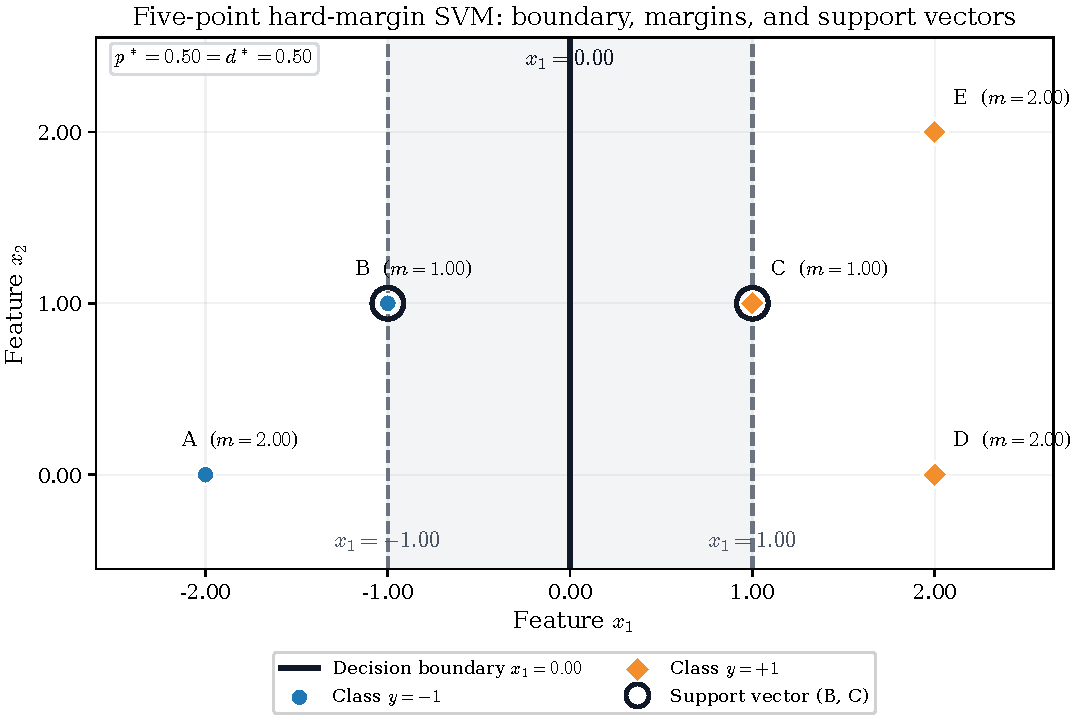
\includegraphics[width=0.92\textwidth]{output/figures/svm_primal_dual_toy_example.pdf}
    \caption{Five-point hard-margin example. The black line is the decision boundary, the dashed lines are the two supporting margins, and the rings identify support vectors B and C. Here $m_i=y_i(w^\top x_i+b)$ denotes the signed functional margin.}
    \label{fig:toy-primal-dual}
\end{figure}

\paragraph{Primal problem and the five constraints.}
For $w=(w_1,\ldots,w_{10})^\top$, the hard-margin primal is
\begin{equation}
\begin{aligned}
\min_{w,b}\quad &\frac12\lVert w\rVert_2^2
   =\frac12\sum_{j=1}^{10}w_j^2\\
\text{subject to}\quad &y_i(w^\top x_i+b)\geq1,
   \qquad i\in\{A,B,C,D,E\}.
\end{aligned}
\end{equation}
Substituting every observation gives
\begin{equation}
\begin{aligned}
\text{A:}\quad
&-1[-2w_1+0w_2+0w_3+\cdots+0w_{10}+b]\geq1
&&\Longleftrightarrow\quad 2w_1-b\geq1,\\
\text{B:}\quad
&-1[-w_1+w_2+0w_3+\cdots+0w_{10}+b]\geq1
&&\Longleftrightarrow\quad w_1-w_2-b\geq1,\\
\text{C:}\quad
&+1[w_1+w_2+0w_3+\cdots+0w_{10}+b]\geq1
&&\Longleftrightarrow\quad w_1+w_2+b\geq1,\\
\text{D:}\quad
&+1[2w_1+0w_2+0w_3+\cdots+0w_{10}+b]\geq1
&&\Longleftrightarrow\quad 2w_1+b\geq1,\\
\text{E:}\quad
&+1[2w_1+2w_2+0w_3+\cdots+0w_{10}+b]\geq1
&&\Longleftrightarrow\quad 2w_1+2w_2+b\geq1.
\end{aligned}
\end{equation}

This is not an unconstrained optimization problem. If one differentiates
only the objective and sets its gradient to zero, then
\begin{equation}
    \nabla_w\left(\frac12\lVert w\rVert_2^2\right)=w=0.
\end{equation}
At $w=0$, the positive-class constraints require $b\geq1$, whereas the
negative-class constraints require $b\leq-1$; no intercept can satisfy both.
The unconstrained minimum is therefore infeasible, which is precisely why
the margin constraints must enter the optimality analysis through the
Lagrangian and KKT conditions.

\paragraph{Solving the primal step by step.}
Add the simplified constraints for B and C:
\begin{equation}
    (w_1-w_2-b)+(w_1+w_2+b)\geq2
    \quad\Longrightarrow\quad w_1\geq1.
\end{equation}
It follows that every feasible point satisfies
\begin{equation}
    \frac12\lVert w\rVert_2^2
    =\frac12(w_1^2+w_2^2+\cdots+w_{10}^2)
    \geq\frac12.
\end{equation}
Choose $w_1=1.00$, $w_2=\cdots=w_{10}=0.00$. The B constraint then gives
$1.00-b\geq1.00$, hence $b\leq0.00$, while the C constraint gives
$1.00+b\geq1.00$, hence $b\geq0.00$. Thus $b=0.00$. This candidate also satisfies
the A, D, and E constraints, so it attains the lower bound and is globally
optimal:
\begin{equation}
    w^*=(1.00,0.00,\ldots,0.00)^\top,\qquad b^*=0.00,
    \qquad p^*=\frac12\lVert w^*\rVert_2^2=0.50.
\end{equation}
The decision equation $(w^*)^\top x+b^*=0$ reduces to $x_1=0.00$.

\begin{table}[htbp]
\centering
\caption{Signed functional margins at the primal optimum.}
\label{tab:toy-margins}
\begin{tabular}{ccccc}
\toprule
Point & $y_i$ & $(w^*)^\top x_i+b^*$ & $y_i((w^*)^\top x_i+b^*)$ & Status \\
\midrule
A & $-1$ & $-2.00$ & $2.00$ & Outside margin \\
B & $-1$ & $-1.00$ & $1.00$ & Support vector \\
C & $+1$ & $1.00$ & $1.00$ & Support vector \\
D & $+1$ & $2.00$ & $2.00$ & Outside margin \\
E & $+1$ & $2.00$ & $2.00$ & Outside margin \\
\bottomrule
\end{tabular}
\end{table}

Table~\ref{tab:toy-margins} confirms that B and C are support vectors because
their signed margins equal $1.00$. A, D, and E have signed margins strictly
greater than $1.00$ and therefore lie outside the margin strip.

\paragraph{Lagrangian, stationarity, and complementary slackness.}
Introduce one multiplier $\alpha_i\geq0$ for each of the five constraints:
\begin{equation}
    \mathcal{L}(w,b,\alpha)
    =\frac12\lVert w\rVert_2^2
    -\sum_{i\in\{A,B,C,D,E\}}
       \alpha_i\left[y_i(w^\top x_i+b)-1\right].
\end{equation}
Stationarity with respect to the primal variables gives
\begin{equation}
\begin{aligned}
\nabla_w\mathcal{L}=0
&\quad\Longrightarrow\quad
w=\sum_i\alpha_i y_i x_i,\\
\frac{\partial\mathcal{L}}{\partial b}=0
&\quad\Longrightarrow\quad
\sum_i\alpha_i y_i=0.
\end{aligned}
\end{equation}
Complementary slackness requires
\begin{equation}
    \alpha_i\left[y_i(w^\top x_i+b)-1\right]=0
    \qquad\text{for every }i.
\end{equation}
For A, D, and E the bracket equals $2.00-1.00=1.00>0$, so complementary
slackness forces
\begin{equation}
    \alpha_A=\alpha_D=\alpha_E=0.00.
\end{equation}
For B and C the bracket is zero, so their multipliers may be positive. The
intercept stationarity equation becomes
\begin{equation}
    -\alpha_B+\alpha_C=0
    \quad\Longrightarrow\quad \alpha_B=\alpha_C=\gamma.
\end{equation}
Substituting this equality into the weight stationarity equation gives
\begin{equation}
\begin{aligned}
w
&=\gamma(-1)(-1,1,0,\ldots,0)
  +\gamma(+1)(1,1,0,\ldots,0)\\
&=(2\gamma,0,\ldots,0).
\end{aligned}
\end{equation}
Matching the primal solution $w^*=(1.00,0.00,\ldots,0.00)$ gives
$2.00\gamma=1.00$, and therefore
\begin{equation}
    \alpha_B=\alpha_C=0.50.
\end{equation}
In the two visible coordinates, the reconstruction is
\begin{equation}
    0.50(-1)(-1.00,1.00)+0.50(+1)(1.00,1.00)=(1.00,0.00),
\end{equation}
which verifies that the two support vectors determine the separating
direction.

\paragraph{Dual problem and strong duality.}
Minimizing the Lagrangian over $w$ and $b$ using the stationarity equations
produces the hard-margin dual
\begin{equation}
\begin{aligned}
\max_{\alpha}\quad
&q(\alpha)=\sum_i\alpha_i
-\frac12\left\lVert\sum_i\alpha_i y_i x_i\right\rVert_2^2\\
\text{subject to}\quad
&\alpha_i\geq0,\qquad \sum_i\alpha_i y_i=0.
\end{aligned}
\end{equation}
For this dataset, the two nonzero coordinates of
$\sum_i\alpha_i y_i x_i$ are
\begin{equation}
\begin{aligned}
z_1&=2\alpha_A+\alpha_B+\alpha_C+2\alpha_D+2\alpha_E,\\
z_2&=-\alpha_B+\alpha_C+2\alpha_E,
\end{aligned}
\end{equation}
so the complete dataset-specific dual is
\begin{equation}
\begin{aligned}
\max_{\alpha\geq0}\quad
&\alpha_A+\alpha_B+\alpha_C+\alpha_D+\alpha_E\\
&\quad-\frac12\left[
(2\alpha_A+\alpha_B+\alpha_C+2\alpha_D+2\alpha_E)^2
 +(-\alpha_B+\alpha_C+2\alpha_E)^2\right]\\
\text{subject to}\quad
&-\alpha_A-\alpha_B+\alpha_C+\alpha_D+\alpha_E=0.
\end{aligned}
\end{equation}
At $(\alpha_A,\alpha_B,\alpha_C,\alpha_D,\alpha_E)
=(0.00,0.50,0.50,0.00,0.00)$, the equality constraint holds and
\begin{equation}
    q(\alpha)
    =0.50+0.50-\frac12[(0.50+0.50)^2+(-0.50+0.50)^2]
    =0.50.
\end{equation}
The primal construction already supplies a feasible value $p^*=0.50$, while
this dual-feasible point supplies the lower bound $d^*=0.50$. Weak duality
prevents a dual value from exceeding a primal value, so equality certifies
that both points are optimal:
\begin{equation}
    \boxed{d^*=0.50=p^*}.
\end{equation}
This zero duality gap is the numerical manifestation of strong duality. The
figure and all calculations in this subsection are reproduced by
\texttt{scripts/build\_svm\_primal\_dual\_toy\_example.py}.

\subsection{Ten-Observation Spreadsheet Illustration}
\label{sec:worked-excel}

To make the matrix constraint concrete, a self-contained teaching table was constructed from the first ten observations in the project spreadsheet. The selection rule is transparent: scan from top to bottom, take the first five UPA and first five BPA observations, and restore source-row order. In this dataset these are exactly rows 2--11. The four hormone variables are log-transformed and all ten features are standardized using statistics from these ten rows. No selected value is missing, so median imputation is inactive.

For $p=10$, the vectors used in one constraint row are
\begin{equation}
    \theta=\begin{bmatrix}w_1&\cdots&w_{10}&b\end{bmatrix}^{\top},
    \qquad
    u_i=t_i\begin{bmatrix}x_{i1}&\cdots&x_{i,10}&1\end{bmatrix}^{\top}.
\end{equation}
Their inner product is the signed functional margin:
\begin{equation}
    u_i^{\top}\theta
    =t_i(x_i^{\top}w+b)
    =t_i s_i.
\end{equation}
The expression is therefore not ``$u_i>1$'': $u_i$ is a vector. The scalar dot product $u_i^{\top}\theta$ must satisfy $u_i^{\top}\theta\geq1$. For UPA, $t_i=+1$ and the rule becomes $s_i\geq1$; for BPA, $t_i=-1$ and it becomes $s_i\leq-1$.

Solving the primal quadratic program for this teaching subsystem gives
\begin{equation}
\begin{aligned}
w_{\mathrm{teach}}^{\top}
\approx{}&(0.34,-0.42,-0.65,0.08,-0.10,\\
&\phantom{(}0.16,-0.13,0.39,-0.75,0.64),\\
b_{\mathrm{teach}}\approx{}&0.29.
\end{aligned}
\end{equation}

\paragraph{Numerical evaluation of the objective.}
The ten observations contribute ten margin constraints; they do not create ten additive loss terms. Thus the fitted teaching subsystem has one global primal objective. Substituting the fitted weights gives
\begin{equation}
\begin{aligned}
\lVert w_{\mathrm{teach}}\rVert_2^2
&\approx (0.34)^2+(-0.42)^2+(-0.65)^2+(0.08)^2+(-0.10)^2\\
&\quad +(0.16)^2+(-0.13)^2+(0.39)^2+(-0.75)^2+(0.64)^2\\
&\approx 1.90\quad\text{from displayed coefficients},\\
&=1.88\quad\text{from full-precision coefficients},\\[2pt]
\phi(\theta_{\mathrm{teach}})
&=\frac12\lVert w_{\mathrm{teach}}\rVert_2^2\\
&=\frac12(1.88)\\
&\approx\boxed{0.94}.
\end{aligned}
\end{equation}
The intercept
$b_{\mathrm{teach}}\approx0.29$ is not squared because the hard-margin primal
does not penalize the intercept. The ten rowwise quantities governed by this
solution are the constraints $u_i^{\top}\theta\geq1$ in
Table~\ref{tab:worked-excel}.

The coefficient order is PAC, PRA, potassium, tumor size, 18-OHF, 18-oxoF, systolic blood pressure, diastolic blood pressure, DDD, and age. Table~\ref{tab:worked-excel} shows every constraint. The complete raw $x_i$, transformed $x_i$, standardized $x_i$, $u_i$, parameter, gradient, and Hessian tables are supplied in the companion CSV folder \texttt{output/csv/hard\_margin\_10row/}.

\begin{table}[htbp]
\centering
\caption{Teaching-only row-by-row evaluation of $u_i^{\top}\theta\geq1$. Displayed values are rounded; feasibility uses unrounded values.}
\label{tab:worked-excel}
\scriptsize
\begin{tabular}{@{}llrrrrcc@{}}
\toprule
Patient & Class & $t_i$ & Score $s_i$ & $u_i^{\top}\theta$ & $g_i=1-u_i^{\top}\theta$ & Feasible & SV \\
\midrule
CGH-001 & UPA & $+1$ &  3.22 & 3.22 & $-2.22$ & Yes & No \\
CGH-002 & UPA & $+1$ &  1.39 & 1.39 & $-0.39$ & Yes & No \\
CGH-003 & UPA & $+1$ &  1.00 & 1.00 &  0.00 & Yes & Yes \\
CGH-004 & BPA & $-1$ & $-1.00$ & 1.00 &  0.00 & Yes & Yes \\
CGH-005 & BPA & $-1$ & $-1.41$ & 1.41 & $-0.41$ & Yes & No \\
CGH-006 & BPA & $-1$ & $-1.59$ & 1.59 & $-0.59$ & Yes & No \\
CGH-007 & BPA & $-1$ & $-1.00$ & 1.00 &  0.00 & Yes & Yes \\
CGH-008 & BPA & $-1$ & $-1.00$ & 1.00 &  0.00 & Yes & Yes \\
CGH-009 & UPA & $+1$ &  2.27 & 2.27 & $-1.27$ & Yes & No \\
CGH-010 & UPA & $+1$ &  1.00 & 1.00 &  0.00 & Yes & Yes \\
\bottomrule
\end{tabular}
\end{table}

For example, CGH-004 is a BPA observation, so $t_4=-1$. Its score is $s_4=-1$, giving $u_4^{\top}\theta=(-1)(-1)=1$ and $g_4=0$. It lies exactly on the negative supporting margin and is a support vector. The corresponding spreadsheet calculation is
\begin{equation}
\begin{aligned}
s_i&=\operatorname{SUMPRODUCT}(x_i,w)+b,\\
u_i^{\top}\theta&=t_i s_i,\\
\text{constraint check}&=(u_i^{\top}\theta\geq1-10^{-8}).
\end{aligned}
\end{equation}

Figure~\ref{fig:worked-scores} plots the raw scores rather than the signed margins. This preserves the two class regions: BPA observations lie at or left of $-1$, UPA observations lie at or right of $+1$, and $s=0$ is the classifier boundary.

\begin{figure}[htbp]
    \centering
    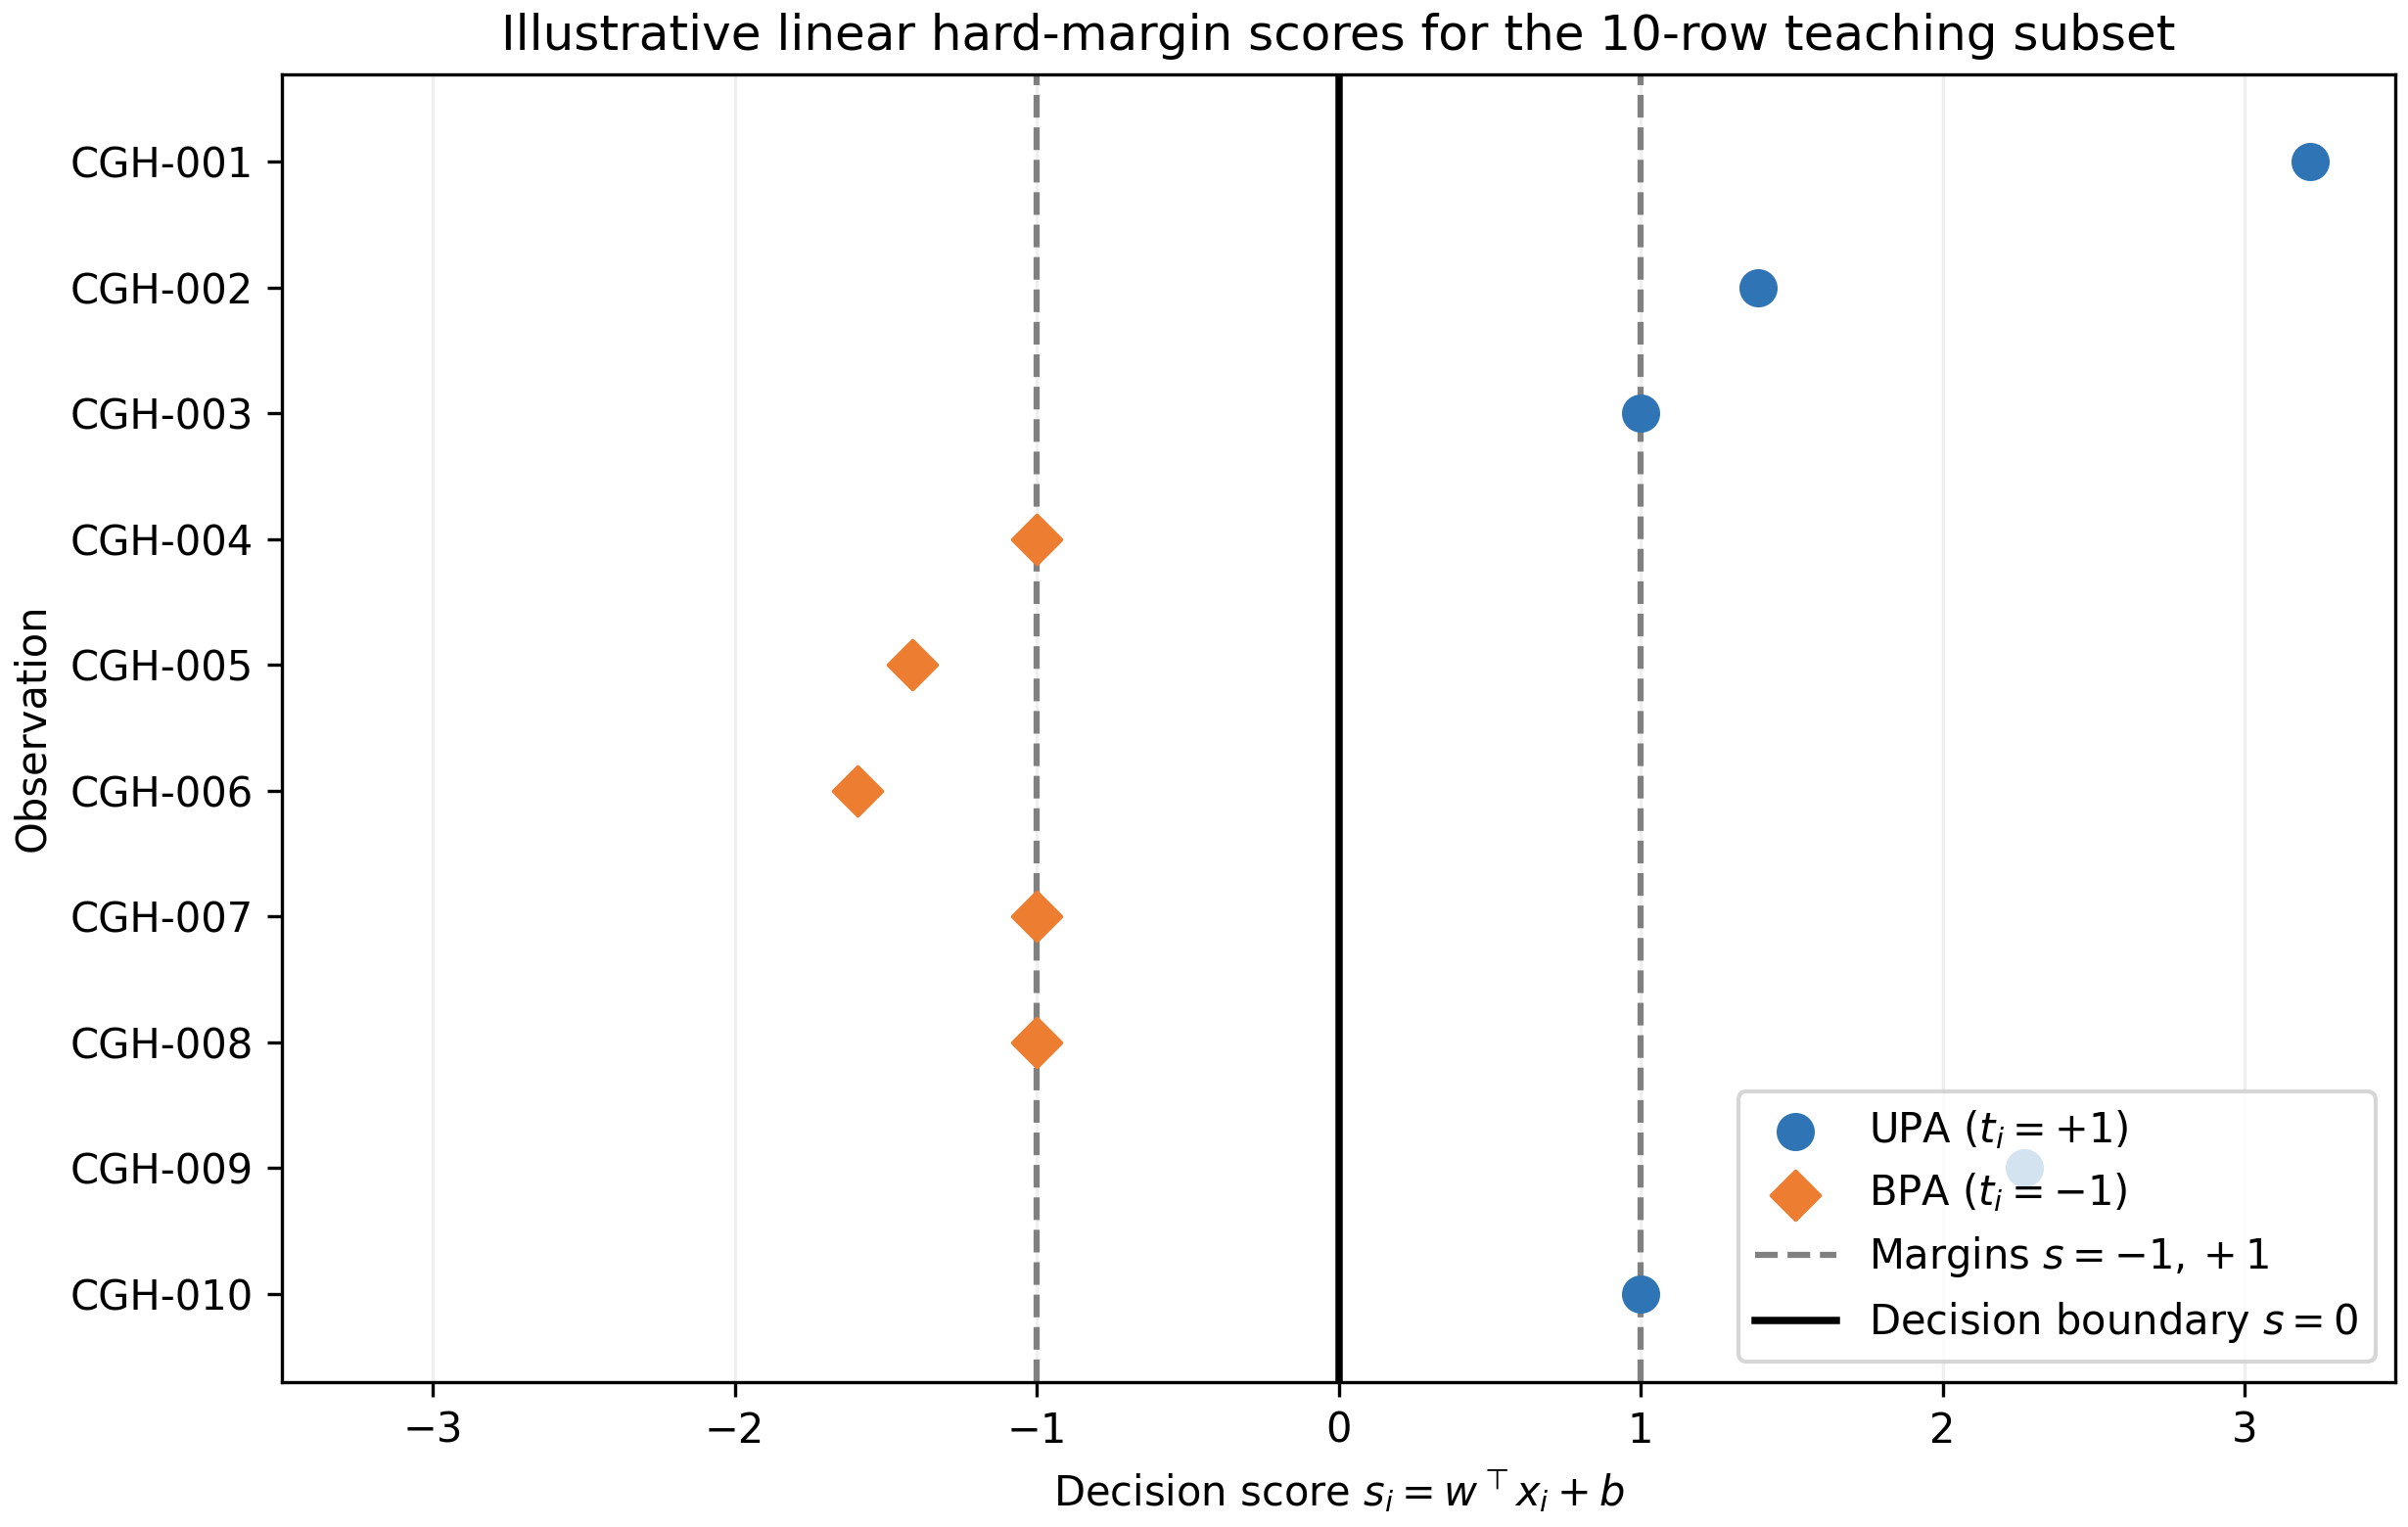
\includegraphics[width=0.92\textwidth]{output/figures/hard_margin_10row_scores.png}
    \caption{Decision scores for the separable ten-row teaching subsystem. This is an algebraic illustration, not a validation or ROC result.}
    \label{fig:worked-scores}
\end{figure}

This feasible subsystem does not imply that the complete cohort is separable. Removing 104 constraints can leave a feasible problem even when adding the remaining constraints makes the full system infeasible. No ROC, AUROC, sensitivity, or specificity is calculated from this ten-row in-sample illustration.

\clearpage
\section{Internal Reproduction and Numerical Audit}
\label{app:verification}

The supplied numerical artifacts were regenerated and audited against the project scripts and
dataset in the local reference environment (Python~3.14, scikit-learn~1.8,
SciPy~1.17, NumPy~2.4, pandas~3.0, Matplotlib~3.10, and openpyxl~3.1).
The corresponding package versions are recorded in
\path{requirements.txt}. Generated full-precision CSV values were compared
against the values reported in the main text.

\begin{itemize}
    \item \textbf{Result tables.} The generated CSV artifacts reproduce the
    reported numerical results. Exact machine-zero residual mantissas can vary
    with summation order and the linear-algebra backend; values below
    $10^{-15}$ are therefore reported as tolerance statements rather than as
    reproducible decimal identities.
    \item \textbf{LaTeX tables.} The displayed table fragments are generated
    directly from their corresponding full-precision CSV artifacts.
    \item \textbf{Figure provenance.} Numerical figures generated by the
    documented scripts are reproducible from the shipped dataset and CSVs.
    Seven explanatory figures are committed static teaching assets:
    \path{feature_distributions}, \path{farkas_lemma_schematic},
    \path{convex_hull_overlap_2d}, \path{fig_step3_c_grid},
    \path{fig_step3_pareto}, \path{fig_step3c_pc_boundary}, and
    \path{fig_step4_rbf_pc_boundary}. They illustrate the same shipped
    calculations but are not claimed as script-generated outputs.
    \item \textbf{Headline metrics.} The linear soft-margin nested
    seed-zero out-of-fold AUROC ($0.9474$), accuracy ($0.8596$), sensitivity
    ($0.8571$), and specificity ($0.8621$), and the RBF selection
    $(C,\gamma)=(0.01,10^{-3})$ with mean outer AUROC $0.9420$, all reproduce
    to six decimal places within the supplied project pipeline. Across twenty
    fold-assignment seeds, the more stable headline means are $0.9401$ for the
    linear SVM and $0.9399$ for the RBF SVM.
    \item \textbf{Optimization quality.} The primal--dual gaps of both fitted
    models are small ($4.9\times10^{-10}$ for the linear model and
    $2.2\times10^{-11}$ for the RBF model), confirming both quadratic programs
    are solved to the stated numerical tolerance.
    \item \textbf{Leakage safety.} The log transformation, median imputation,
    and standardization are all contained inside the cross-validation
    pipeline, so every preprocessing parameter is estimated from the training
    fold alone. The nested cross-validation is therefore free of information
    leakage.
\end{itemize}

The primary conclusion is confirmed: the RBF kernel did not provide a stable
improvement over the linear soft-margin model. With only 114 observations and
substantial overlap among repeated splits, the fold and seed repetitions are
treated as validation and stability diagnostics rather than independent
replicates for formal significance testing. Preferring the simpler linear
model is therefore the supported, appropriately cautious conclusion.

\section{Source Code}
\label{app:code}

All code, the synthetic dataset, and the generated figures and tables are
available in the project repository:
\begin{center}
\url{https://github.com/nttssv/convex_optimization_svm_example}
\end{center}

The repository is organized as follows. Each script is reached by appending
its path to
\path{https://github.com/nttssv/convex_optimization_svm_example/blob/main/}.

\begin{itemize}
    \item \path{scripts/linear_hard_margin_svm.py} --- fold-wise
    preprocessing, the hard-margin feasibility test by linear programming, and
    the constrained primal solve used in Section~\ref{sec:hard-margin}.
    \item \path{scripts/linear_soft_margin_svm.py} --- leakage-safe nested
    cross-validation, selection of $C$ by AUROC, the final soft-margin fit with
    its primal--dual audit, and the tables and figures of
    Section~\ref{sec:soft-margin}.
    \item \path{scripts/compare_primal_optimizers.py} --- controlled comparison
    of stochastic subgradient, Heavy Ball momentum-subgradient, and
    Nesterov-style momentum-subgradient methods in Section~\ref{sec:sgm}.
    \item \path{scripts/kernel_rbf_svm.py} --- joint $C,\gamma$ tuning inside
    nested cross-validation, the train--validation gap diagnostic, and the
    RBF-versus-linear comparison of Section~\ref{sec:kernel-rbf}.
    \item \path{scripts/build_full_data_infeasibility_certificate.py} --- the
    Farkas infeasibility certificate of Section~\ref{sec:full-certificate}.
    \item \path{scripts/build_descriptive_tables.py} --- the descriptive
    statistics and class-contrast tables of Section~\ref{sec:descriptive}.
    \item \path{scripts/build_svm_primal_dual_toy_example.py} --- the
    five-point primal--dual teaching example in Appendix~\ref{sec:toy-primal-dual}.
    \item \path{scripts/build_hard_margin_teaching_workbook.py} --- the
    ten-observation teaching subsystem and companion spreadsheet.
    \item \path{scripts/build_seed_robustness.py} --- the repeated-seed
    stability diagnostic comparing the linear and RBF models.
    \item \path{scripts/build_boundary_sensitivity.py} --- the explicitly
    post-selection audit of the lower $C$ and $\gamma$ grid boundaries.
    \item \path{scripts/build_baseline_comparison.py} --- twenty-seed PAC-only,
    L2-logistic, linear-SVM, and RBF-SVM context comparison.
    \item \path{scripts/make_synthetic_dataset.py} --- deterministic
    generation of the synthetic input cohort from seed $20260710$.
    \item \path{scripts/_pubstyle.py} --- shared plotting style used by the
    publication figures.
    \item Legacy exploratory utilities (unused by every headline result, table,
    and figure): \path{scripts/svm_convergence.py};\\
    \path{scripts/svm_cv_eval.py}; and\\
    \path{scripts/svm_diagnostics_from_data.py}.
    \item \path{data/cgh_pa_dataset.csv} --- the synthetic 114-patient cohort;
    \path{output/} --- the regenerated figures, CSV audits, and \LaTeX{} table
    fragments.
\end{itemize}

The exact execution order and PDF-build command are documented in
\path{README.md}. Running those commands from the repository root, with
\path{scripts/} on \texttt{PYTHONPATH}, regenerates the report's tables,
numerical audit files, and script-produced figures. The seven static teaching
figures listed above are shipped directly in \path{output/figures/}.

\end{document}
